\documentclass[11pt]{article}
\usepackage[margin=1in]{geometry}
\usepackage[T1]{fontenc}
\usepackage[utf8]{inputenc}
\usepackage{lmodern}
\usepackage{microtype}
\usepackage{hyperref}
\usepackage{xurl}
\usepackage{booktabs}
\usepackage{longtable}
\usepackage{array}
\usepackage{listings}
\usepackage{xcolor}
\usepackage{enumitem}
\usepackage{caption}
\usepackage{pgfplots}
\usepackage[section]{placeins}
\usepackage{algpseudocode}

\pgfplotsset{compat=1.18}
\usetikzlibrary{arrows.meta,positioning,fit}
\setlength{\tabcolsep}{4pt}
\setlength{\emergencystretch}{2em}

\hypersetup{
  colorlinks=true,
  linkcolor=blue,
  urlcolor=blue,
  citecolor=blue,
  pdftitle={flutter\_kiwi\_nlp: A Native-First Cross-Platform Korean NLP Plugin for Flutter},
  pdfauthor={Jai-Chang Park}
}

\newcolumntype{L}[1]{>{\raggedright\arraybackslash}p{#1}}

\lstdefinestyle{code}{
  basicstyle=\ttfamily\small,
  keywordstyle=\bfseries,
  commentstyle=\itshape,
  breaklines=true,
  frame=single,
  columns=fullflexible,
  keepspaces=true,
  showstringspaces=false
}
\algrenewcommand\algorithmicrequire{\textbf{Input:}}
\algrenewcommand\algorithmicensure{\textbf{Output:}}

\title{\textbf{flutter\_kiwi\_nlp: A Native-First, Cross-Platform Korean NLP Plugin for Flutter}}
\author{Jai-Chang Park\thanks{Google Developer Expert (GDE), Dart \& Flutter; GDG (Google Developer Groups) Golang Korea; Flutter Seoul.}}
\date{February 18, 2026}

\begin{document}
\maketitle

\begin{abstract}
This paper presents \texttt{flutter\_kiwi\_nlp}, a production-oriented
Flutter plugin for Korean morphological analysis built on Kiwi. The package
exposes one stable Dart API while internally operating two runtime stacks:
Native (Dart FFI + C bridge + Kiwi shared library) and Web
(Dart JS interop + kiwi-nlp WASM). This design enables a single application
codebase across Android, iOS, macOS, Linux, Windows, and Web.
Unlike ONNX-export deployment paths, this integration does not require adding
an extra generic inference runtime layer because Kiwi already provides the
analysis engine and model format used here.

The implementation is explicitly aligned with on-device AI requirements:
local inference execution, reduced text egress by default, predictable latency
without per-request network dependence, and operational fallback controls for
model provisioning. Empirically, repeated benchmark trials show that Flutter
throughput is lower than the Python-native baseline in current measurements:
approximately 0.72x on same-host desktop baseline, and as low as 0.63x in
mobile engineering-reference rows that compare emulator/simulator Flutter runs
against host macOS Python. The updated benchmark pipeline also adds boundary-
decomposed measurements (pure processing vs full JSON path), quantifying
serialization/parsing overhead at 11--15\% of Flutter full-path elapsed time
across measured environments. Cross-runtime linguistic agreement remains close on
gold corpora
(88.39\% vs 88.58\% token agreement; 84.90\% vs 85.55\% POS agreement).
On native targets, inference can run fully offline after one-time model
provisioning.

This paper provides an implementation-complete, reproducible specification of
API contract, runtime parity rules, build automation hooks, security boundaries,
failure taxonomy, benchmark protocol, and quantified ecosystem survey signals.
\end{abstract}

\section{Introduction}
Korean morphological analysis is a foundational primitive for search, retrieval,
classification, and generation workflows. In Flutter environments, application
logic can be shared across targets, but language runtime integration remains
platform-specific. \texttt{flutter\_kiwi\_nlp} addresses this mismatch by
encapsulating runtime diversity behind a single API boundary.

The central engineering problem is not only to expose Kiwi functionality, but to
make runtime behavior predictable when deployment environments differ in:

\begin{itemize}[leftmargin=1.5em]
  \item native dynamic library semantics,
  \item browser module and WASM loading constraints,
  \item model-file availability,
  \item platform build toolchains and artifact formats.
\end{itemize}

\subsection{On-Device AI Positioning}
This plugin is designed as an on-device AI integration layer, not a
network-first inference client. In this context, "on-device" means that
tokenization and morphological analysis execute inside the host application
process (native FFI path) or in-browser runtime (WASM path), with optional
model download only for provisioning. This positioning provides:
\begin{itemize}[leftmargin=1.5em]
  \item stronger default data locality for analyzed text,
  \item lower dependency on network availability during inference,
  \item deterministic runtime behavior under explicit model/version controls,
  \item easier integration into privacy- or compliance-sensitive workloads.
\end{itemize}

For native targets, once model artifacts are bundled or cached locally, analysis
can execute without network connectivity (offline-first inference path). For web
targets, comparable offline behavior requires deployment-specific caching and
self-hosting policy because the default bootstrap uses CDN module/WASM URLs.

\subsection{Contribution Type}
This paper is positioned as a \textbf{systems/resource} contribution rather than
an algorithmic NLP paper. Its primary value is integration engineering:
cross-runtime API unification, deterministic fallback policy, reproducible
benchmark protocol, and deployable build/runtime controls for Flutter
applications. It does not claim a new morphological decoding algorithm or a new
Korean language model architecture.

\section{Related Work}
This revision expands the related-work coverage to include core Transformer
foundations, compact/efficient variants, on-device inference studies, and
Korean-language-specific resources. For foundation and compression lineage,
prior work includes BERT, ALBERT, ELECTRA, DistilBERT, TinyBERT, MiniLM, and
MobileBERT
\cite{ref_bert,ref_albert,ref_electra,ref_distilbert,ref_tinybert,ref_minilm,ref_mobilebert}.
These studies establish the main trade-off surface between representational
quality and model size/latency.

For edge execution and deployment-oriented efficiency, SqueezeBERT, EdgeBERT,
and DeeBERT provide architectural or runtime pathways for lower-latency
transformer inference, while pNLP-Mixer explores an all-MLP design for compact
on-device language modeling
\cite{ref_squeezebert,ref_edgebert,ref_deebert,ref_pnlp_mixer}. Application
focused on-device work reports practical workloads such as VQA, form filling,
and smart-reply code-switching, and personalization-oriented studies analyze
device-local vocabulary adaptation under memory/latency constraints
\cite{ref_on_device_apps,ref_personalized_vocab}.

For Korean NLP context, KR-BERT, KLUE, KoBigBird-large, and character-level
Korean morphological analysis/POS tagging provide complementary evidence on
language-specific tokenization, evaluation, and modeling behavior
\cite{ref_kr_bert,ref_klue,ref_kobigbird,ref_korean_morph_pos}. These works are
primarily model or benchmark contributions; by contrast, this paper focuses on
systems integration for production Flutter apps, including runtime selection,
artifact provisioning, fallback semantics, and reproducibility constraints.

The Korean morphological analyzer ecosystem itself is also important related
work context. Widely used dictionary-centric analyzers and lexicons such as
MeCab-ko and MeCab-ko-dic represent a practical baseline in many production
pipelines, while Khaiii represents a neural approach with different quality and
runtime trade-offs \cite{ref_mecab_ko,ref_mecab_ko_dic,ref_khaiii}. In Python
workflows, KoNLPy is often used as an integration layer over multiple Korean
analyzers, affecting how researchers compare or operationalize analyzers in
practice \cite{ref_konlpy}. Relative to that landscape, this paper's main
contribution is not proposing a new Korean analyzer itself, but delivering a
native-first, cross-platform Flutter integration path for Kiwi with explicit
reproducibility and deployment controls.

Table~\ref{tab:korean-analyzer-landscape} summarizes commonly used Korean
morphological analyzers/toolkits in practice, with repository-level adoption
signals collected on February 17, 2026 via GitHub API snapshots
\cite{ref_github_rest}.

\begingroup
\footnotesize
\setlength{\tabcolsep}{3pt}
\begin{longtable}{@{}L{0.14\linewidth}L{0.15\linewidth}L{0.25\linewidth}L{0.30\linewidth}L{0.10\linewidth}@{}}
\caption{Representative Korean morphological analyzers and usage landscape (snapshot: 2026-02-17)}\label{tab:korean-analyzer-landscape}\\
\toprule
Analyzer / Toolkit & Primary runtime & Typical usage context & Adoption signal (snapshot) & Source \\
\midrule
\endfirsthead
\toprule
Analyzer / Toolkit & Primary runtime & Typical usage context & Adoption signal (snapshot) & Source \\
\midrule
\endhead
Kiwi & Native C++ (+ wrappers) & Production morphology/POS pipelines; offline embedding & GitHub stars: 671 & \cite{ref_kiwi_repo} \\

MeCab-ko (+ mecab-ko-dic) & Native C++ & Established tokenization/POS baseline; commonly used via KoNLPy Mecab path & MeCab upstream + Eunjeon lineage references; no canonical active GitHub org repo in this snapshot & \cite{ref_mecab_ko,ref_mecab_ko_dic,ref_konlpy} \\

Khaiii & Native C++/Python wrapper & Neural Korean analyzer for batch/server usage & GitHub stars: 1,448 & \cite{ref_khaiii} \\

Open Korean Text (Okt) & JVM/Scala (+ wrappers) & Social-text normalization/tokenization in JVM and Python workflows & GitHub stars: 656 & \cite{ref_open_korean_text,ref_konlpy} \\

KOMORAN & JVM & Java production pipelines and KoNLPy-integrated experiments & GitHub stars: 311 & \cite{ref_komoran_repo,ref_konlpy} \\

KoNLPy (toolkit) & Python wrapper hub & Unified interface over Kkma, Hannanum, Komoran, Mecab, Okt & GitHub stars: 1,486 & \cite{ref_konlpy,ref_konlpy_repo} \\
\bottomrule
\end{longtable}
\endgroup

For benchmark methodology, GLUE and SuperGLUE establish widely reused
task-oriented NLU evaluation structure, and Long Range Arena targets efficiency
comparison under long-context settings
\cite{ref_glue,ref_superglue,ref_lra}. For systems-level performance reporting,
DAWNBench and MLPerf Inference provide complementary protocol ideas such as
time-to-accuracy framing and cross-stack inference benchmarking
\cite{ref_dawnbench,ref_mlperf_inference}.

From a systems perspective, on-device ML discussions increasingly emphasize
data locality, reduced dependency on always-on connectivity, and deployment
practicality under edge constraints \cite{ref_tinyml}. These themes align with
the operational goals of \texttt{flutter\_kiwi\_nlp}: local inference path,
deterministic runtime controls, and explicit provisioning/fallback mechanisms.

Privacy-preserving distributed training literature such as FedAvg also informs
the broader motivation for keeping user data local when possible
\cite{ref_fedavg}. Although this plugin targets inference rather than training,
the same locality principle reinforces its offline-first native execution model.

\section{Background: Flutter and Kiwi}
\subsection{What Flutter Is}
Flutter is an open-source UI toolkit for building applications from one Dart
codebase across mobile, desktop, and web targets. Its rendering and widget
model allows large parts of application logic to be shared, but low-level
platform integration is still target-specific.

For systems like NLP analyzers, Flutter integration typically requires one of:
\begin{itemize}[leftmargin=1.5em]
  \item platform channels (message-based bridge), or
  \item FFI plugins (direct native library interop from Dart).
\end{itemize}

\texttt{flutter\_kiwi\_nlp} uses FFI for native platforms and JS interop on web,
which is why the plugin architecture is more complex than standard UI-only
Flutter packages.

\subsection{What Dart Is and Why It Was Created}
Dart is an open-source, client-optimized language developed by Google and used
as the language foundation of Flutter. The Dart project positions the language
goal as productive multi-platform development paired with a flexible runtime
platform.\footnote{\url{https://dart.dev/overview}}

The practical reason this matters for plugin engineering is that Dart is
designed for both development-time velocity and production deployment across
multiple backends. In current official language positioning, this includes:
\begin{itemize}[leftmargin=1.5em]
  \item fast iterative development workflows (for example, hot-reload-oriented
  tooling in Flutter),
  \item ahead-of-time native compilation for device/desktop targets, and
  \item web-target compilation paths (JavaScript and WebAssembly).\footnote{
  \url{https://dart.dev/}}
\end{itemize}

For this plugin, these Dart properties directly motivate the design choice to
publish one stable Dart API while internally dispatching to platform-specific
runtime backends.

\subsection{What Rust Is and Why It Is Mentioned}
Rust is an open-source systems programming language designed around memory
safety, strong compile-time guarantees, and predictable performance without a
garbage collector.\footnote{\url{https://www.rust-lang.org/}}

This repository is not primarily implemented in Rust: native runtime integration
here is built on a Dart FFI layer and a C bridge that loads Kiwi artifacts.
Rust is still worth documenting in this paper because reviewers often ask about
Rust's role in modern WebAssembly ecosystems. In this plugin, consumer builds do
not require a Rust toolchain; web execution depends on the distributed
\texttt{kiwi-nlp} JS/WASM artifacts and native execution depends on platform
libraries.
This is an intentional interoperability tradeoff: the package prioritizes
adopting upstream Kiwi distribution artifacts over introducing an additional
language toolchain requirement for plugin consumers.

\subsection{What WebAssembly (WASM) Is}
WebAssembly (WASM) is a compact binary instruction format and execution model
for stack-based virtual machines.\footnote{\url{https://webassembly.org/}}
On the web it runs inside the browser sandbox, typically loaded by JavaScript
bootstrap code, and enables near-native computational kernels while preserving
browser security constraints.

In plugin context, WASM is not a replacement for Flutter itself; it is a backend
execution target used by the web runtime path to execute Kiwi analysis logic in
browser environments.

\subsection{What Kiwi Is}
Kiwi is a Korean morphological analysis engine distributed primarily as a native
library and ecosystem artifacts. In this repository, Kiwi is consumed through:
\begin{itemize}[leftmargin=1.5em]
  \item native dynamic libraries loaded by a C bridge on Android/iOS/macOS/Linux/Windows,
  \item the \texttt{kiwi-nlp} JavaScript/WASM package on web.
\end{itemize}

Operationally, Kiwi performs segmentation and POS-tagged token analysis, and
the plugin exposes that capability as:
\texttt{create}, \texttt{analyze}, \texttt{addUserWord}, and \texttt{close}.

Model files are external artifacts (for example \texttt{cong.mdl},
\texttt{default.dict}, \texttt{typo.dict}) that must be present locally,
packaged as Flutter assets, or obtained through archive fallback.

\subsubsection{How Kiwi Models Are Trained (Upstream Summary)}
Kiwi's upstream design separates dictionary/rule-driven candidate generation
from statistical disambiguation. In practical terms, this means model training
is centered on language-model estimation over morphologically analyzed corpora,
while lexicon/rule components remain explicit resources
\cite{ref_kiwi_repo,ref_kiwi_paper}.

Upstream documentation and the Kiwi paper describe training data composition
using large Korean morphological corpora, including Sejong and National
Institute of Korean Language resources, and report model-family evolution from
KNLM-focused scoring to Skip-Bigram and contextual n-gram embedding variants
\cite{ref_kiwi_repo,ref_kiwi_paper}.

For \texttt{flutter\_kiwi\_nlp}, the operational implication is explicit:
this package consumes prebuilt Kiwi model artifacts for inference, and does not
re-implement Kiwi training in the Flutter build/runtime path.

\subsubsection{Kiwi Internal Architecture (From Upstream Source)}
Upstream Kiwi implementation and public headers indicate that runtime decoding
is organized as a morphology candidate graph/lattice search with language-model
scoring, rather than a Transformer encoder stack
\cite{ref_kiwi_repo,ref_kiwi_types_h,ref_kiwi_kiwi_h,ref_kiwi_path_evaluator}.
At the API/type level, model families are explicitly defined as:
\texttt{knlm} (Kneser--Ney LM), \texttt{sbg} (Skip-Bigram), and
\texttt{cong/congGlobal} (contextual N-gram embedding LM variants), with no
Transformer model type in the exposed enum
\cite{ref_kiwi_types_h}.

At inference-time, Kiwi keeps LM state while evaluating candidate paths over
the morpheme graph and applies additional rule-based penalties/bonuses for
morphological compatibility and punctuation/quote state handling
\cite{ref_kiwi_kiwi_h,ref_kiwi_path_evaluator}. This is closer to a
graph-decoding + statistical language-model architecture than to deep
self-attention sequence encoding.

\subsubsection{Conceptual Decoding Objective}
For reviewer readability, the upstream behavior can be summarized as a lattice
path optimization problem (conceptual/illustrative form; not a claim of
reproducing every internal constant/feature exactly):
\[
\pi^{*}=\mathop{\mathrm{arg\,max}}_{\pi\in\Pi(G)} S(\pi),
\]
where \(G\) is the morpheme lattice and \(\Pi(G)\) is the set of valid paths.
The path score is composed additively:
\[
S(\pi)=\sum_{t=1}^{T(\pi)}
\left[
s_{\mathrm{lm}}(e_t,h_{t-1})
\;+\;
\lambda^{\top}\phi_{\mathrm{rule}}(e_t,c_t)
\;+\;
\gamma^{\top}\phi_{\mathrm{lex}}(e_t)
\right].
\]
Here, \(e_t\) denotes the selected candidate edge at step \(t\), \(h_{t-1}\) is
the LM state carried from prior steps, \(c_t\) encodes local context such as
quote/punctuation conditions, and \(\phi_{\mathrm{rule}},\phi_{\mathrm{lex}}\)
represent rule/lexicon-derived feature contributions.

State progression and pruning can be abstracted as:
\[
h_t=F(h_{t-1},e_t),\qquad
\mathcal{B}_t=\mathrm{TopK}\!\left(\mathcal{P}_t(G),K_{\mathrm{beam}},S\right),
\]
where \(\mathcal{P}_t(G)\) is the partial-path set at depth \(t\), and
\(\mathcal{B}_t\) is the retained beam-like frontier with width
\(K_{\mathrm{beam}}\).

The LM-family switch exposed by Kiwi model type can be written as:
\[
s_{\mathrm{lm}}=
\left\{
\begin{array}{ll}
s_{\mathrm{knlm}}, & m=\mathrm{knlm}, \\
s_{\mathrm{knlm}}+\Delta_{\mathrm{sbg}}, & m=\mathrm{sbg}, \\
s_{\mathrm{cong}}, & m=\mathrm{cong}, \\
s_{\mathrm{cong\mbox{-}global}}, & m=\mathrm{congGlobal}.
\end{array}
\right.
\]
This formulation explains why Kiwi behaves as graph decoding with explicit LM
state and rule scoring, rather than Transformer self-attention inference.

\subsubsection{Skip-Bigram and Contextual N-gram Scoring (Conceptual)}
Because the plugin references Kiwi model families \texttt{sbg} and
\texttt{cong/congGlobal}, it is useful to provide explicit conceptual scoring
forms for reviewer intuition:
\[
\Delta_{\mathrm{sbg}}(e_t,h_{t-1})
\approx
\sum_{k=1}^{\min(K_{\mathrm{skip}},t-1)}\alpha_k\,
\psi_k\!\left(m_t,m_{t-k}\right),
\]
where \(m_t\) is the morpheme realized by edge \(e_t\), \(k\) is skip distance,
and \(\alpha_k\) is a distance-dependent weight.
The function \(\psi_k\) denotes skip-bigram interaction score components.
Here \(K_{\mathrm{skip}}\) is the maximum skip order considered.

A generic contextual n-gram embedding style score can be expressed as:
\[
c_t=\sum_{j=1}^{\min(n-1,t-1)}W_j\,v(m_{t-j}),\qquad
s_{\mathrm{cong}}(e_t,h_{t-1})\approx u(m_t)^{\top}c_t+b(m_t),
\]
where \(v(\cdot)\) and \(u(\cdot)\) denote context/target embeddings and
\(W_j\) encodes positional/context projection.

For the long-context variant, a practical abstraction is:
\[
c_t^{\mathrm{global}}=\sum_{j=1}^{\min(n_g-1,t-1)}W_j^{(g)}\,v(m_{t-j}),\qquad
s_{\mathrm{cong\mbox{-}global}}(e_t,h_{t-1})
\approx
u(m_t)^{\top}c_t^{\mathrm{global}}+b_g(m_t),
\]
with \(n_g > n\) to reflect wider context coverage.

These equations are intentionally presented as conceptual abstractions to
explain model-family behavior at paper level; exact implementation constants and
feature composition are defined by upstream Kiwi internals and model artifacts.
They are explanatory model-family formulations and are not used directly to
compute the benchmark tables in Section~\ref{tab:benchmark}.

Figure~\ref{fig:kiwi-internal-architecture} summarizes this upstream-oriented
view of Kiwi internals as used in the plugin context.

\begin{figure}[htbp]
\centering
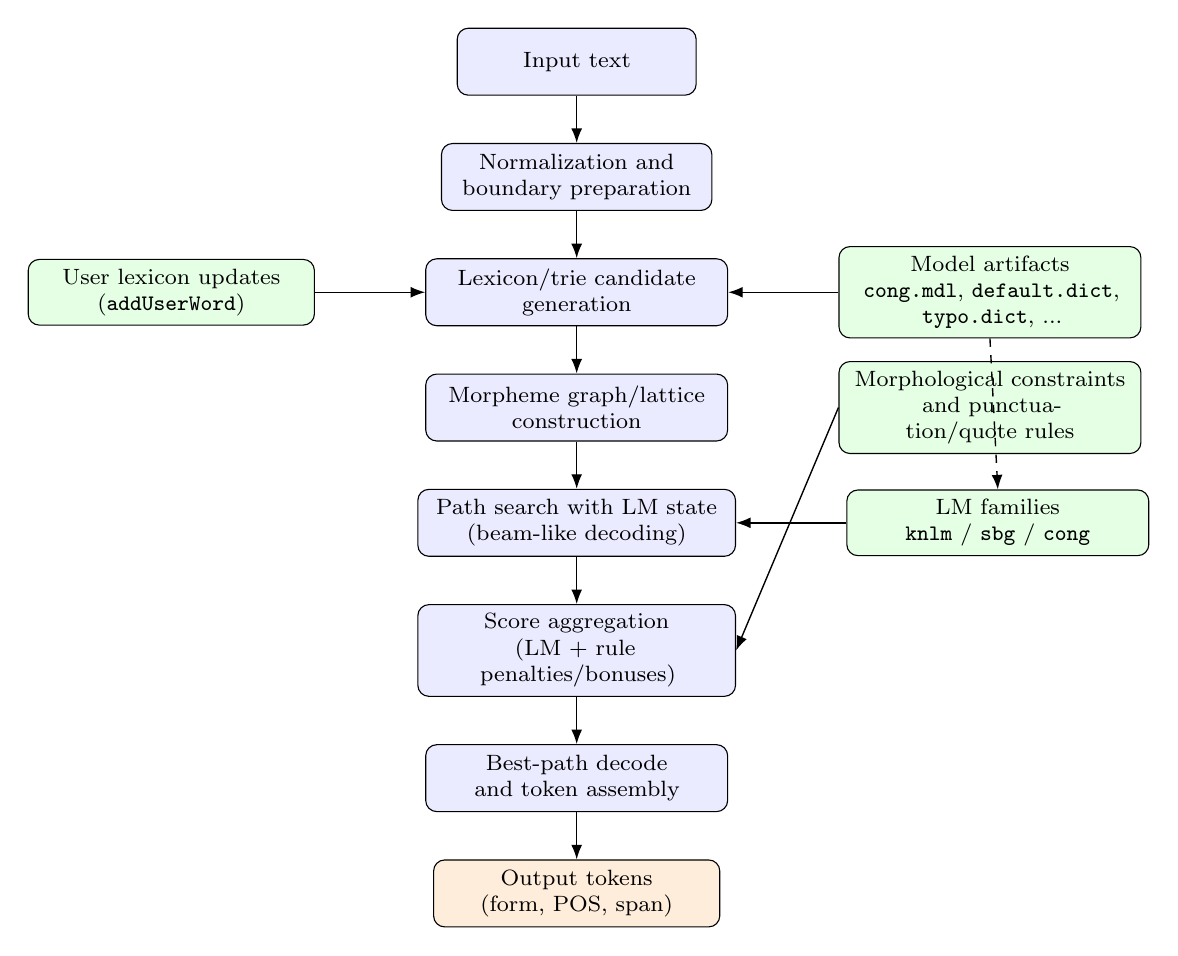
\begin{tikzpicture}[
  >=Latex,
  node distance=6mm and 8mm,
  phase/.style={
    draw,
    rounded corners,
    align=center,
    font=\footnotesize,
    minimum height=8.5mm,
    fill=blue!8
  },
  resource/.style={
    draw,
    rounded corners,
    align=center,
    font=\footnotesize,
    minimum height=8mm,
    fill=green!10
  },
  arr/.style={->, line width=0.5pt}
]
\node[phase, text width=28mm] (input) {Input text};
\node[phase, text width=32mm, below=of input] (normalize)
{Normalization and\\boundary preparation};
\node[phase, text width=36mm, below=of normalize] (candidate)
{Lexicon/trie candidate\\generation};
\node[phase, text width=36mm, below=of candidate] (lattice)
{Morpheme graph/lattice\\construction};
\node[phase, text width=38mm, below=of lattice] (search)
{Path search with LM state\\(beam-like decoding)};
\node[phase, text width=38mm, below=of search] (score)
{Score aggregation\\(LM + rule penalties/bonuses)};
\node[phase, text width=36mm, below=of score] (decode)
{Best-path decode\\and token assembly};
\node[phase, text width=34mm, below=of decode, fill=orange!14] (output)
{Output tokens\\(form, POS, span)};

\node[resource, text width=36mm, right=14mm of candidate] (models)
{Model artifacts\\\texttt{cong.mdl}, \texttt{default.dict},\\\texttt{typo.dict}, ...};
\node[resource, text width=36mm, right=14mm of lattice] (constraints)
{Morphological constraints\\and punctuation/quote rules};
\node[resource, text width=36mm, right=14mm of search] (lmfamily)
{LM families\\\texttt{knlm} / \texttt{sbg} / \texttt{cong}};
\node[resource, text width=34mm, left=14mm of candidate] (userlex)
{User lexicon updates\\(\texttt{addUserWord})};

\draw[arr] (input) -- (normalize);
\draw[arr] (normalize) -- (candidate);
\draw[arr] (candidate) -- (lattice);
\draw[arr] (lattice) -- (search);
\draw[arr] (search) -- (score);
\draw[arr] (score) -- (decode);
\draw[arr] (decode) -- (output);

\draw[arr] (models.west) -- (candidate.east);
\draw[arr] (constraints.west) -- (score.east);
\draw[arr] (lmfamily.west) -- (search.east);
\draw[arr] (userlex.east) -- (candidate.west);
\draw[arr, dashed] (models.south) -- (lmfamily.north);
\end{tikzpicture}
\caption{Conceptual Kiwi internal architecture based on upstream source
inspection.}
\label{fig:kiwi-internal-architecture}
\end{figure}

\subsubsection{Why This Is Not a Transformer}
Transformer-based analyzers typically center on stacked self-attention blocks
and dense neural sequence representations. Kiwi's upstream architecture, by
contrast, is designed around:
\begin{itemize}[leftmargin=1.5em]
  \item lexicon/trie-driven candidate generation and morphological constraints,
  \item explicit path search with LM-state progression over candidates,
  \item lightweight N-gram-family scoring models (\texttt{knlm/sbg/cong}).
\end{itemize}

This distinction explains why Kiwi integration characteristics differ from
Transformer runtimes: lower footprint and predictable CPU inference behavior are
prioritized, while broad semantic representation power is not the primary design
target in this component.

\subsubsection{Why No ONNX Runtime Layer Is Required}
Some modern NLP deployment stacks package neural models in ONNX format and
ship an additional generic runtime engine (for example, ONNX Runtime) inside
the application process. \texttt{flutter\_kiwi\_nlp} intentionally does not
add that extra layer, because Kiwi already provides its own inference/decode
engine and model format for Korean morphological analysis.

This design choice has practical implications:
\begin{itemize}[leftmargin=1.5em]
  \item fewer runtime components to integrate and version-lock,
  \item simpler build/runtime dependency surface for plugin consumers,
  \item no separate ONNX operator/runtime compatibility matrix to maintain.
\end{itemize}

Important scope clarification: this is a dependency and integration argument,
not a universal speed claim against all ONNX-based analyzers. In this paper's
own benchmark, \texttt{flutter\_kiwi\_nlp} still trails Python-native
\texttt{kiwipiepy} throughput due to bridge overhead, even though the backend
engine itself is Kiwi in both cases.

\subsection{Why This Integration Is Non-Trivial}
The plugin is not a direct wrapper around one runtime. It is an orchestration
layer that has to keep semantics stable across different execution models:
\begin{itemize}[leftmargin=1.5em]
  \item native C ABI with explicit memory ownership,
  \item browser JS/WASM with promise-based async semantics,
  \item platform-specific build systems and artifact formats.
\end{itemize}

\section{Prior Ecosystem Survey: Existing Kiwi Wrappers}
\subsection{Survey Scope and Method}
This paper includes an explicit prior-ecosystem survey to position
\texttt{flutter\_kiwi\_nlp} against existing Kiwi bindings. The survey source is
the upstream Kiwi repository README and linked binding projects, plus GitHub
repository metadata snapshots collected on February 17, 2026.\footnote{
\url{https://github.com/bab2min/Kiwi}}

\subsection{Observed Upstream Wrapper/Binding Landscape}
Table~\ref{tab:kiwi-survey} summarizes the wrappers and binding channels
explicitly referenced upstream.

\begin{longtable}{@{}L{0.19\linewidth}L{0.25\linewidth}L{0.50\linewidth}@{}}
\caption{Upstream Kiwi wrapper/binding survey (as documented by Kiwi)}\label{tab:kiwi-survey}\\
\toprule
Category & Location & Notes \\
\midrule
\endfirsthead
\toprule
Category & Location & Notes \\
\midrule
\endhead
C API & \path{include/kiwi/capi.h} & Core C interface for native embedding. \\

Prebuilt binaries & Kiwi releases page & Windows/Linux/macOS/Android library and model artifacts are distributed through release assets. \\

C\# wrapper (official GUI usage) & \url{https://github.com/bab2min/kiwi-gui} & Upstream points to C\# wrapper used by official GUI tooling. \\

C\# wrapper (community) & \url{https://github.com/EX3exp/NetKiwi} & Community-contributed multiplatform C\# wrapper linked by upstream README. \\

Python wrapper & \url{https://github.com/bab2min/kiwipiepy} & Officially documented Python3 API package. \\

Java binding & \path{bindings/java} in Kiwi repository & Java 1.8+ binding path documented upstream. \\

Android library & Kiwi release asset (\path{kiwi-android-VERSION.aar}) & Android NDK-based AAR distribution path documented upstream. \\

R wrapper & \url{https://mrchypark.github.io/elbird/} & Community-contributed R wrapper linked by upstream README. \\

Go wrapper & \url{https://github.com/codingpot/kiwigo} & Community Go wrapper linked by upstream README. \\

WebAssembly binding & \path{bindings/wasm} in Kiwi repository & JavaScript/TypeScript-facing WASM binding path documented upstream. \\
\bottomrule
\end{longtable}

\subsection{Gap Analysis and Motivation for This Work}
The upstream survey shows broad language coverage around Kiwi, but it also
shows a practical integration gap for Flutter package consumers:
\begin{itemize}[leftmargin=1.5em]
  \item no upstream-listed first-class Dart/Flutter wrapper entry,
  \item no upstream-listed packaging path that unifies native (mobile/desktop)
  and web (WASM) behind one Dart API contract,
  \item no upstream-listed Flutter-specific build-hook automation for shipping
  platform artifacts in plugin workflows.
\end{itemize}

This gap is the direct motivation for \texttt{flutter\_kiwi\_nlp}: one
Flutter-native package that preserves Kiwi backend capability while adding
runtime abstraction, model resolution policy, and target-specific packaging
automation needed by real Flutter deployments.

\subsection{Quantified Maintenance Signals}
To reduce purely descriptive bias, this revision adds repository-level
maintenance signals collected from GitHub REST API snapshots on
February 17, 2026 (\path{tool/benchmark/collect_wrapper_activity.py}).
Table~\ref{tab:kiwi-survey-quant} reports latest release date, latest commit
date, and commit velocity windows for each wrapper repository.

\begin{table}[htbp]
\centering
\small
\caption{Quantified wrapper maintenance signals (as-of 2026-02-17)}
\label{tab:kiwi-survey-quant}
\begin{tabular}{@{}L{0.12\linewidth}L{0.20\linewidth}L{0.14\linewidth}L{0.14\linewidth}L{0.08\linewidth}L{0.08\linewidth}L{0.06\linewidth}@{}}
\toprule
Wrapper & Repo & Latest release & Last commit & 90d commits & 365d commits & Stars \\
\midrule
kiwi-gui & \path{bab2min/kiwi-gui} & 2025-12-22 (57d) & 2025-12-22 (57d) & 10 & 18 & 14 \\
NetKiwi & \path{EX3exp/NetKiwi} & N/A & 2025-02-18 (364d) & 0 & 1 & 2 \\
kiwipiepy & \path{bab2min/kiwipiepy} & 2025-12-15 (64d) & 2025-12-25 (54d) & 33 & 114 & 357 \\
Kiwi Java binding & \path{bab2min/Kiwi} & 2025-12-15 (64d) & 2026-02-02 (15d) & 30 & 279 & 671 \\
Kiwi WASM binding & \path{bab2min/Kiwi} & 2025-12-15 (64d) & 2026-02-02 (15d) & 30 & 279 & 671 \\
elbird & \path{mrchypark/elbird} & 2025-12-30 (49d) & 2025-12-30 (49d) & 37 & 44 & 34 \\
kiwigo & \path{codingpot/kiwigo} & N/A & 2025-10-15 (125d) & 0 & 5 & 30 \\
\bottomrule
\end{tabular}
\end{table}

\begin{figure}[htbp]
\centering
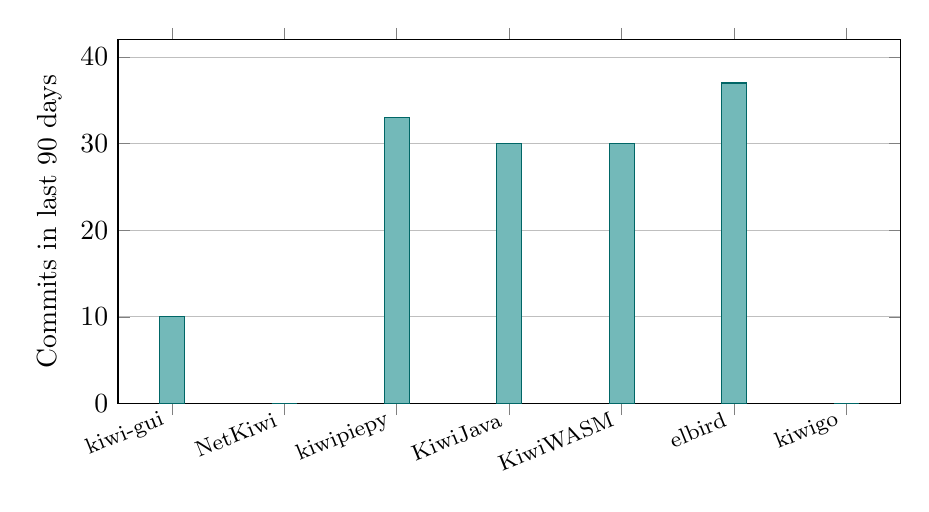
\begin{tikzpicture}
\begin{axis}[
  ybar,
  bar width=9pt,
  width=0.95\linewidth,
  height=6.2cm,
  ymin=0,
  ymax=42,
  ymajorgrids=true,
  ylabel={Commits in last 90 days},
  symbolic x coords={kiwi-gui,NetKiwi,kiwipiepy,KiwiJava,KiwiWASM,elbird,kiwigo},
  xtick=data,
  x tick label style={font=\footnotesize, rotate=22, anchor=east},
  enlarge x limits=0.08
]
\addplot+[
  fill=teal!55,
  draw=teal!80!black
] coordinates {
  (kiwi-gui,10)
  (NetKiwi,0)
  (kiwipiepy,33)
  (KiwiJava,30)
  (KiwiWASM,30)
  (elbird,37)
  (kiwigo,0)
};
\end{axis}
\end{tikzpicture}
\caption{Recent wrapper activity (90-day commit count).}
\label{fig:wrapper-commits-90d}
\end{figure}

\begin{figure}[htbp]
\centering
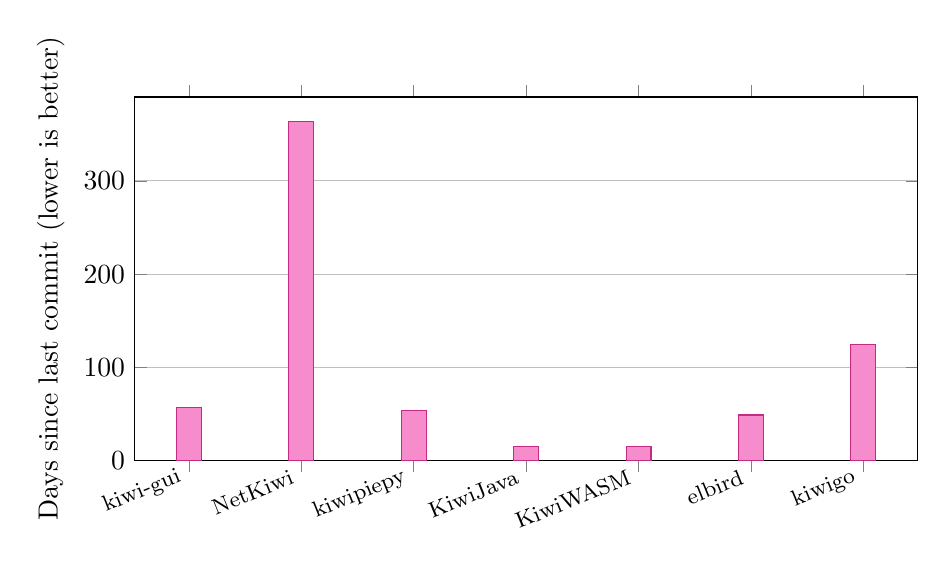
\begin{tikzpicture}
\begin{axis}[
  ybar,
  bar width=9pt,
  width=0.95\linewidth,
  height=6.2cm,
  ymin=0,
  ymax=390,
  ymajorgrids=true,
  ylabel={Days since last commit (lower is better)},
  symbolic x coords={kiwi-gui,NetKiwi,kiwipiepy,KiwiJava,KiwiWASM,elbird,kiwigo},
  xtick=data,
  x tick label style={font=\footnotesize, rotate=22, anchor=east},
  enlarge x limits=0.08
]
\addplot+[
  fill=magenta!45,
  draw=magenta!80!black
] coordinates {
  (kiwi-gui,57)
  (NetKiwi,364)
  (kiwipiepy,54)
  (KiwiJava,15)
  (KiwiWASM,15)
  (elbird,49)
  (kiwigo,125)
};
\end{axis}
\end{tikzpicture}
\caption{Repository recency profile for upstream wrappers.}
\label{fig:wrapper-recency-days}
\end{figure}

\subsection{Survey Evidence Limits}
These maintenance signals are repository-level proxies. For Java and WASM, the
metrics come from the shared Kiwi monorepo and do not isolate directory-level
binding effort. Issue response latency and download velocity are also not yet
included.

\section{Design Goals and Non-Goals}
\subsection{Primary Goals}
\begin{enumerate}[leftmargin=1.5em]
  \item \textbf{Stable API contract}: identical Dart signatures across native,
  web, and unsupported stubs.
  \item \textbf{Operational resilience}: layered model resolution, archive
  fallback, and explicit error propagation.
  \item \textbf{Build-time ergonomics}: automatic preparation of missing Kiwi
  artifacts during platform builds.
  \item \textbf{Typed outputs}: deterministic output schema
  (result \textrightarrow{} candidates \textrightarrow{} tokens).
\end{enumerate}

\subsection{Explicit Non-Goals}
\begin{itemize}[leftmargin=1.5em]
  \item Novel morphological-analysis algorithm or model-training contribution.
  \item Full feature parity with every upstream Kiwi API detail.
  \item Guaranteed throughput parity with Python-native \texttt{kiwipiepy}.
  \item Support for targets not declared in Flutter plugin metadata
  (for example, Fuchsia).
\end{itemize}

\section{Supported Platform Matrix}
Table~\ref{tab:platform-matrix} summarizes currently supported targets,
execution backend, artifact strategy, and packaging hook.

\begin{longtable}{@{}L{0.10\linewidth}L{0.13\linewidth}L{0.13\linewidth}L{0.18\linewidth}L{0.34\linewidth}@{}}
\caption{Current platform support matrix}\label{tab:platform-matrix}\\
\toprule
Platform & Flutter plugin declaration & Runtime backend & Bundled artifact & Preparation hook \\
\midrule
\endfirsthead
\toprule
Platform & Flutter plugin declaration & Runtime backend & Bundled artifact & Preparation hook \\
\midrule
\endhead
Android & Supported (\texttt{ffiPlugin}) & Native FFI + C bridge + \texttt{libkiwi.so} & \path{android/src/main/jniLibs/<abi>/libkiwi.so} & Gradle task \texttt{prepareKiwiAndroidLibs} bound to \texttt{preBuild} \\

iOS & Supported (\texttt{ffiPlugin}) & Native FFI + C bridge + Kiwi framework & \path{ios/Frameworks/Kiwi.xcframework} & Podspec hook (\texttt{prepare\_command}) runs \path{tool/build_ios_kiwi_xcframework.sh} \\

macOS & Supported (\texttt{ffiPlugin}) & Native FFI + C bridge + libkiwi & \path{macos/Frameworks/libkiwi.dylib} & Podspec hook (\texttt{prepare\_command}) runs \path{tool/build_macos_kiwi_dylib.sh} \\

Linux & Supported (\texttt{ffiPlugin}) & Native FFI + C bridge + \texttt{libkiwi.so} & \path{linux/prebuilt/libkiwi.so} & CMake custom target \texttt{prepare\_kiwi\_linux\_lib} \\

Windows & Supported (\texttt{ffiPlugin}) & Native FFI + C bridge + \texttt{kiwi.dll} & \path{windows/prebuilt/kiwi.dll} & CMake custom target \texttt{prepare\_kiwi\_windows\_dll} \\

Web & Supported (web plugin class) & JS interop + \texttt{kiwi-nlp} WASM & Model files loaded by URL or archive bytes in memory & Runtime module/model loader in \path{kiwi_analyzer_web.dart} \\

Fuchsia & Not declared & Stub behavior & N/A & N/A \\
\bottomrule
\end{longtable}

\subsection{Architecture Coverage}
\begin{itemize}[leftmargin=1.5em]
  \item Android ABIs default to \texttt{arm64-v8a} and \texttt{x86\_64}.
  \item iOS framework build includes \texttt{iphoneos arm64} and simulator
  \texttt{arm64/x86\_64} slices.
  \item macOS default build targets \texttt{arm64} and \texttt{x86\_64}.
  \item Linux supports host-driven architecture mapping
  (\texttt{x86\_64}, \texttt{arm64}, \texttt{ppc64le}) in build scripts.
  \item Windows arch normalization supports \texttt{x64} (\texttt{x86\_64}),
  \texttt{Win32} (\texttt{x86}), and \texttt{arm64}; prebuilt download path
  currently covers \texttt{x64}/\texttt{Win32}.
\end{itemize}

\subsection{Artifact Footprint Snapshot}
Table~\ref{tab:artifact-footprint} summarizes build/model size signals that are
already tracked in project documentation and re-checked from workspace artifacts
for this revision. These are engineering reference numbers, not final
store-delivery APK/IPA install sizes.

\begin{table}[htbp]
\centering
\small
\caption{Artifact footprint snapshot (workspace measurement, 2026-02-18)}
\label{tab:artifact-footprint}
\begin{tabular}{@{}L{0.42\linewidth}L{0.17\linewidth}L{0.35\linewidth}@{}}
\toprule
Artifact & Size (approx.) & Notes \\
\midrule
Default model directory (\path{assets/kiwi-models/cong/base}) & 99,308,057 bytes (\(\approx\)94.71MiB) & Uncompressed model files used by the plugin. \\
Same default model compressed as local \texttt{.tgz} archive & 79,494,329 bytes (\(\approx\)75.8MiB) & Local compression reference from this workspace. \\
\path{android/src/main/jniLibs/arm64-v8a/libkiwi.so} & 166,229,088 bytes (\(\approx\)158.53MiB) & Current artifact is \texttt{with debug\_info}, \texttt{not stripped}. \\
\path{android/src/main/jniLibs/x86\_64/libkiwi.so} & 200,071,656 bytes (\(\approx\)190.80MiB) & Current artifact is \texttt{with debug\_info}, \texttt{not stripped}. \\
\bottomrule
\end{tabular}
\end{table}

To avoid ambiguity between source artifacts and packaged binaries,
Table~\ref{tab:artifact-footprint-apk} reports example Android app outputs for
both debug and release builds in the same workspace snapshot.

\begin{table}[htbp]
\centering
\small
\caption{Example Android package footprint (debug vs release, 2026-02-18)}
\label{tab:artifact-footprint-apk}
\begin{tabular}{@{}L{0.42\linewidth}L{0.17\linewidth}L{0.35\linewidth}@{}}
\toprule
Packaged item & Size & Notes \\
\midrule
\path{example/build/app/outputs/flutter-apk/app-debug.apk} & 178,454,872 bytes (\(\approx\)170.19MiB) & Example app debug APK. \\
\path{example/build/app/outputs/flutter-apk/app-release.apk} & 113,030,559 bytes (\(\approx\)107.80MiB) & Example app release APK. \\
Release APK entry \path{lib/arm64-v8a/libkiwi.so} & 7,613,192 bytes & Stripped native library entry inside APK. \\
Release APK entry \path{lib/x86_64/libkiwi.so} & 11,381,344 bytes & Stripped native library entry inside APK. \\
Release APK model entries \path{assets/.../kiwi-models/cong/base/*} & 79,574,759 bytes compressed & Same files are 99,308,057 bytes uncompressed. \\
\bottomrule
\end{tabular}
\end{table}

Interpretation notes:
\begin{itemize}[leftmargin=1.5em]
  \item Compressed and uncompressed measurements are not directly comparable.
  \item Source-tree native binaries and packaged APK entries represent different
  pipeline stages.
  \item Android packaging strips debug symbols from native libraries in this
  build flow, which dominates the source-vs-packaged size gap.
  \item ABI-specific native binaries should be interpreted per target split.
  \item Final store-delivery size can further differ by app-bundle splitting and
  distribution-side compression.
\end{itemize}

\section{Public API Specification}
\subsection{Entry Point and Conditional Export}
Public package entry point is \texttt{lib/flutter\_kiwi\_nlp.dart}. Runtime
selection uses conditional exports:

\begin{lstlisting}[style=code]
export 'src/kiwi_analyzer_stub.dart'
    if (dart.library.io) 'src/kiwi_analyzer_native.dart'
    if (dart.library.js_interop) 'src/kiwi_analyzer_web.dart';
\end{lstlisting}

This guarantees a single import path for consumers while allowing runtime-
specific implementation files.

\subsection{Core Analyzer API}
Table~\ref{tab:core-api} lists the complete analyzer surface exposed to users.

\begin{longtable}{@{}L{0.34\linewidth}L{0.62\linewidth}@{}}
\caption{Core public analyzer API}\label{tab:core-api}\\
\toprule
Signature & Contract \\
\midrule
\endfirsthead
\toprule
Signature & Contract \\
\midrule
\endhead
\texttt{static Future<KiwiAnalyzer> create(...)} & Creates analyzer instance. Parameters include model path inputs, build/match flags, and thread count. Native resolves model path and opens FFI handle; web imports module and builds Kiwi instance (with fallback); stub throws unsupported exception. \\

\texttt{String get nativeVersion} & Returns backend version string. Native reads bridge-provided version. Web prefixes with \texttt{web/wasm}. Stub returns unsupported message. \\

\texttt{Future<KiwiAnalyzeResult> analyze(String text, \{KiwiAnalyzeOptions options\})} & Runs morphological analysis with candidate count and match options. Returns typed result object. Throws \texttt{KiwiException} on runtime failure or use-after-close. \\

\texttt{Future<void> addUserWord(String word, \{String tag='NNP', double score=0.0\})} & Registers user dictionary entry. Native invokes bridge function directly. Web stores word and rebuilds analyzer with accumulated \texttt{userWords}. \\

\texttt{Future<void> close()} & Releases resources and closes instance. Native closes bridge handle; web clears in-memory state; repeated use after close is rejected. \\
\bottomrule
\end{longtable}

\subsection{Options and Flags API}
\subsubsection{\texttt{KiwiBuildOption} constants}
\begin{longtable}{@{}L{0.40\linewidth}L{0.54\linewidth}@{}}
\caption{Build option flags}\label{tab:build-flags}\\
\toprule
Constant & Meaning \\
\midrule
\endfirsthead
\toprule
Constant & Meaning \\
\midrule
\endhead
\texttt{integrateAllomorph} & Enable allomorph integration. \\
\texttt{loadDefaultDict} & Load default dictionary. \\
\texttt{loadTypoDict} & Load typo dictionary. \\
\texttt{loadMultiDict} & Load multi-word dictionary. \\
\texttt{modelTypeDefault} & Use backend default model type. \\
\texttt{modelTypeLargest} & Select largest model variant. \\
\texttt{modelTypeKnlm} & Select KNLM model variant. \\
\texttt{modelTypeSbg} & Select SBG model variant. \\
\texttt{modelTypeCong} & Select CONG model variant. \\
\texttt{modelTypeCongGlobal} & Select global CONG variant. \\
\texttt{defaultOption} & Recommended bundle:
\texttt{integrateAllomorph | loadDefaultDict | loadTypoDict |
loadMultiDict | modelTypeCong}. \\
\bottomrule
\end{longtable}

\subsubsection{\texttt{KiwiMatchOption} constants}
\begin{longtable}{@{}L{0.38\linewidth}L{0.56\linewidth}@{}}
\caption{Match option flags}\label{tab:match-flags}\\
\toprule
Constant & Meaning \\
\midrule
\endfirsthead
\toprule
Constant & Meaning \\
\midrule
\endhead
\texttt{url}, \texttt{email}, \texttt{hashtag}, \texttt{mention}, \texttt{serial} & Detect corresponding token classes. \\
\texttt{normalizeCoda} & Normalize final consonants. \\
\texttt{joinNounPrefix}, \texttt{joinNounSuffix}, \texttt{joinVerbSuffix}, \texttt{joinAdjSuffix}, \texttt{joinAdvSuffix} & Join morphology according to POS-specific rules. \\
\texttt{splitComplex} & Split complex forms. \\
\texttt{zCoda} & Enable coda-related matching behavior. \\
\texttt{compatibleJamo} & Emit compatibility jamo style output. \\
\texttt{splitSaisiot}, \texttt{mergeSaisiot} & Control sai-sios split/merge behavior. \\
\texttt{all} & Baseline option bundle. \\
\texttt{allWithNormalizing} & \texttt{all} plus \texttt{normalizeCoda}. \\
\bottomrule
\end{longtable}

\subsubsection{\texttt{KiwiAnalyzeOptions}}
\texttt{KiwiAnalyzeOptions} carries request-level options:
\texttt{topN} (candidate count) and \texttt{matchOptions} (bitwise flags).

\subsection{Result and Exception Models}
\begin{longtable}{@{}L{0.32\linewidth}L{0.62\linewidth}@{}}
\caption{Public model types}\label{tab:model-types}\\
\toprule
Type & Fields and semantics \\
\midrule
\endfirsthead
\toprule
Type & Fields and semantics \\
\midrule
\endhead
\texttt{KiwiToken} & \texttt{form}, \texttt{tag}, offsets
(\texttt{start}, \texttt{length}), positions
(\texttt{wordPosition}, \texttt{sentPosition}), confidence metrics
(\texttt{score}, \texttt{typoCost}). \\

\texttt{KiwiCandidate} & \texttt{probability} and ordered
\texttt{List<KiwiToken>} sequence. \\

\texttt{KiwiAnalyzeResult} & \texttt{List<KiwiCandidate>} candidates. \\

\texttt{KiwiException} & User-facing failure wrapper with message string;
used for runtime, model, and lifecycle failures. \\
\bottomrule
\end{longtable}

\section{System Architecture Overview}
Figure~\ref{fig:plugin-architecture} summarizes how one Dart API fans out into
native and web runtime lanes while preserving a shared contract.

\begin{figure}[htbp]
\centering
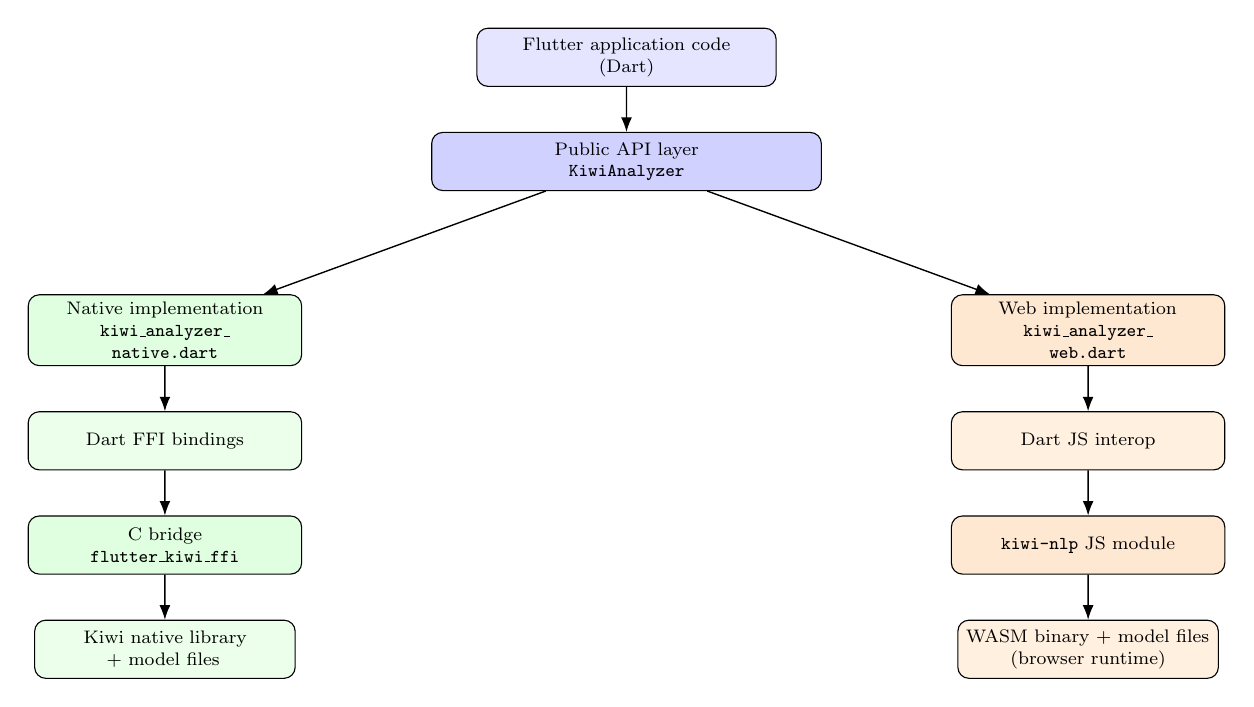
\begin{tikzpicture}[scale=0.82, transform shape,
  >=Latex,
  node distance=7mm and 10mm,
  box/.style={
    draw,
    rounded corners,
    align=center,
    font=\footnotesize,
    minimum height=9mm,
    fill=gray!8
  },
  core/.style={box, fill=blue!10, text width=44mm},
  lane/.style={box, text width=40mm},
  leaf/.style={box, text width=38mm},
  arr/.style={->, line width=0.5pt}
]
\node[core] (app) {Flutter application code\\(Dart)};
\node[core, below=of app, fill=blue!18, text width=58mm] (api)
{Public API layer\\\texttt{KiwiAnalyzer}};

\node[lane, below left=16mm and 20mm of api, fill=green!12] (n1)
{Native implementation\\\texttt{kiwi\_analyzer\_}\\\texttt{native.dart}};
\node[lane, below=of n1, fill=green!8] (n2)
{Dart FFI bindings};
\node[lane, below=of n2, fill=green!12] (n3)
{C bridge\\\texttt{flutter\_kiwi\_ffi}};
\node[leaf, below=of n3, fill=green!8] (n4)
{Kiwi native library\\+ model files};

\node[lane, below right=16mm and 20mm of api, fill=orange!18] (w1)
{Web implementation\\\texttt{kiwi\_analyzer\_}\\\texttt{web.dart}};
\node[lane, below=of w1, fill=orange!12] (w2)
{Dart JS interop};
\node[lane, below=of w2, fill=orange!18] (w3)
{\texttt{kiwi-nlp} JS module};
\node[leaf, below=of w3, fill=orange!12] (w4)
{WASM binary + model files\\(browser runtime)};

\draw[arr] (app) -- (api);
\draw[arr] (api) -- (n1);
\draw[arr] (api) -- (w1);
\draw[arr] (n1) -- (n2);
\draw[arr] (n2) -- (n3);
\draw[arr] (n3) -- (n4);
\draw[arr] (w1) -- (w2);
\draw[arr] (w2) -- (w3);
\draw[arr] (w3) -- (w4);
\end{tikzpicture}
\caption{High-level plugin architecture\\for native and web paths.}
\label{fig:plugin-architecture}
\end{figure}

\subsection{Architecture Reading Notes}
\begin{itemize}[leftmargin=1.5em]
  \item The API entrypoint is intentionally singular (\texttt{KiwiAnalyzer}) to
  keep application code independent from target runtime.
  \item Native and web lanes diverge below the API surface, then converge back
  to the same typed Dart result models.
  \item Model artifacts remain external data assets in both lanes, but loading
  strategies differ by runtime constraints.
\end{itemize}

\section{Native Runtime Implementation}
\subsection{Layered Architecture}
Native execution is deliberately split into three layers:

\begin{enumerate}[leftmargin=1.5em]
  \item Dart analyzer implementation
  (\texttt{lib/src/kiwi\_analyzer\_native.dart}).
  \item C bridge shared library
  (\texttt{src/flutter\_kiwi\_ffi.c}, header
  \texttt{src/flutter\_kiwi\_ffi.h}).
  \item Kiwi shared library (loaded dynamically by the bridge).
\end{enumerate}

Dart calls generated bindings in
\path{lib/flutter_kiwi_ffi_bindings_generated.dart}; the bridge owns
Kiwi symbol resolution and native error buffering.

\subsection{Bridge ABI}
The bridge exports a compact ABI:
\texttt{init}, \texttt{close}, \texttt{analyze\_json},
\texttt{add\_user\_word}, \texttt{free\_string},
\texttt{last\_error}, and \texttt{version}.

The key design choice is JSON transport for analyze output. This decouples Dart
from Kiwi internal structs and simplifies ownership management across language
boundaries.

Initial JSON adoption was also a delivery-speed choice during early plugin
bring-up. The analyzer output is a nested, variable-length schema
(results/candidates/tokens), and a JSON boundary allowed stable cross-language
representation before introducing a custom binary schema/allocator contract.
In practical terms, the initial trade-off prioritized:
\begin{itemize}[leftmargin=1.5em]
  \item schema evolution safety across bridge and Dart model changes,
  \item lower early risk for pointer-ownership bugs in nested payload paths,
  \item straightforward debugging with human-readable payloads.
\end{itemize}
The benchmark sections show the cost of that choice explicitly: measurable
serialization overhead on hot paths, motivating binary/typed bridge evolution.

\subsection{Dart FFI Binding Layer}
The native path uses Dart's \texttt{dart:ffi} for symbol binding and
\texttt{package:ffi/ffi.dart} for UTF-8/pointer utilities. At runtime:
\begin{enumerate}[leftmargin=1.5em]
  \item \path{lib/src/kiwi_analyzer_native.dart} opens the bridge dynamic library.
  \item \path{lib/flutter_kiwi_ffi_bindings_generated.dart} binds exported C symbols.
  \item \texttt{GeneratedKiwiNativeBindings} adapts generated calls behind the
  \texttt{KiwiNativeBindings} interface for testability and swap-in fakes.
\end{enumerate}

This structure keeps API code independent from raw pointer handling while still
using zero-copy native handles for analyzer lifecycle management.

\subsubsection{FFI Type/Ownership Mapping}
\begin{itemize}[leftmargin=1.5em]
  \item \texttt{flutter\_kiwi\_ffi\_handle\_t*} $\rightarrow$
  opaque \texttt{Pointer<flutter\_kiwi\_ffi\_handle\_t>} in Dart.
  \item \texttt{int32\_t} and \texttt{float} $\rightarrow$
  Dart \texttt{int}/\texttt{double} via generated \texttt{asFunction()} bridges.
  \item \texttt{char*} inputs are allocated from Dart strings, passed as UTF-8,
  and explicitly released on the Dart side.
  \item \texttt{char*} outputs from \texttt{analyze\_json()} are bridge-owned and
  must be released by \path{flutter_kiwi_ffi_free_string()}.
  \item Error text from \path{last_error()} is thread-local on the bridge side
  and consumed as read-only C strings from Dart.
\end{itemize}

\subsection{ffigen Generation Pipeline}
Binding code is generated (not handwritten) from the canonical header
\path{src/flutter_kiwi_ffi.h}. The generation source-of-truth is
\path{ffigen.yaml}, which declares:
\begin{itemize}[leftmargin=1.5em]
  \item binding class name: \texttt{FlutterKiwiFfiBindings},
  \item entry/include header: \path{src/flutter_kiwi_ffi.h},
  \item output file: \path{lib/flutter_kiwi_ffi_bindings_generated.dart}.
\end{itemize}

Regeneration command:
\begin{lstlisting}[style=code]
dart run ffigen --config ffigen.yaml
\end{lstlisting}

Why this paper uses \texttt{ffigen} instead of handwritten bindings:
\begin{itemize}[leftmargin=1.5em]
  \item ABI drift resistance when C signatures evolve in
  \path{src/flutter_kiwi_ffi.h}.
  \item Deterministic regeneration from one header/config pair, which improves
  reviewability and incident forensics.
  \item Lower human error risk in repetitive signature plumbing
  (\texttt{NativeFunction}, \texttt{asFunction()}, pointer type mapping).
  \item Consistent symbol surface between C exports and Dart binding class.
  \item \texttt{FlutterKiwiFfiBindings} keeps explicit bridge/API mapping and
  lowers long-term maintenance risk across Android/iOS/desktop targets.
\end{itemize}

\subsubsection{Code-Generation Pipeline Diagram}
\begin{figure}[htbp]
\centering
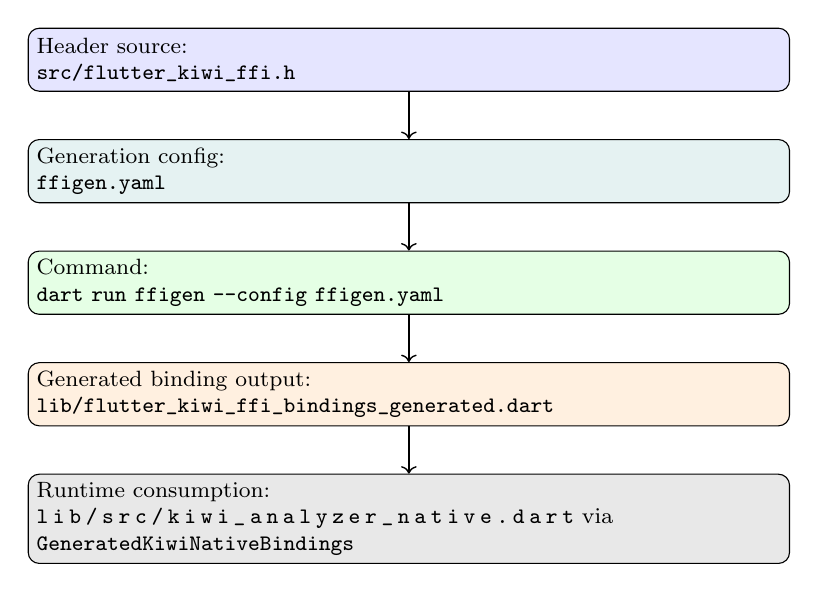
\begin{tikzpicture}[
  node distance=6mm,
  flow/.style={
    draw,
    rounded corners,
    align=left,
    font=\footnotesize,
    text width=0.78\linewidth,
    fill=gray!8,
    minimum height=8mm,
    inner sep=3pt
  },
  arr/.style={->, line width=0.5pt}
]
\node[flow, fill=blue!10] (h) {Header source:\\\path{src/flutter_kiwi_ffi.h}};
\node[flow, below=of h, fill=teal!10] (c) {Generation config:\\\path{ffigen.yaml}};
\node[flow, below=of c, fill=green!10] (cmd) {Command:\\\texttt{dart run ffigen --config ffigen.yaml}};
\node[flow, below=of cmd, fill=orange!12] (out) {Generated binding output:\\\path{lib/flutter_kiwi_ffi_bindings_generated.dart}};
\node[flow, below=of out, fill=gray!18] (use) {Runtime consumption:\\\path{lib/src/kiwi_analyzer_native.dart} via \texttt{GeneratedKiwiNativeBindings}};
\draw[arr] (h) -- (c);
\draw[arr] (c) -- (cmd);
\draw[arr] (cmd) -- (out);
\draw[arr] (out) -- (use);
\end{tikzpicture}
\caption{Dart FFI code-generation pipeline used in this plugin.}
\label{fig:ffigen-pipeline}
\end{figure}

\subsection{Dynamic Library Loading Strategy}
\subsubsection{Bridge loading (Dart side)}
Candidate library names are tried in order by host platform:

\begin{itemize}[leftmargin=1.5em]
  \item Apple: \path{flutter_kiwi_nlp.framework/flutter_kiwi_nlp}, then
  \path{flutter_kiwi_ffi.framework/flutter_kiwi_ffi}.
  \item Linux/Android: \texttt{libflutter\_kiwi\_ffi.so}, then
  \texttt{libflutter\_kiwi\_nlp.so}.
  \item Windows: \texttt{flutter\_kiwi\_ffi.dll}, then
  \texttt{flutter\_kiwi\_nlp.dll}.
\end{itemize}

\subsubsection{Kiwi engine loading (C bridge side)}
Bridge logic accepts optional override path via environment:
\path{FLUTTER_KIWI_NLP_LIBRARY_PATH}
(legacy alias: \path{FLUTTER_KIWI_FFI_LIBRARY_PATH}).
Errors are captured in thread-local storage and exposed through
\texttt{flutter\_kiwi\_ffi\_last\_error()}.

\subsection{Analyzer Lifecycle and Memory Ownership}
\subsubsection{Creation}
\begin{enumerate}[leftmargin=1.5em]
  \item Resolve model directory using layered strategy.
  \item Convert path to UTF-8 pointer.
  \item Call \texttt{flutter\_kiwi\_ffi\_init(...)}.
  \item On null handle, read bridge error and throw \texttt{KiwiException}.
  \item Free temporary path pointer.
\end{enumerate}

\subsubsection{Analysis}
\begin{enumerate}[leftmargin=1.5em]
  \item Ensure analyzer is open.
  \item Convert input string to UTF-8 pointer.
  \item Call \texttt{flutter\_kiwi\_ffi\_analyze\_json}.
  \item Decode JSON into \texttt{KiwiAnalyzeResult}.
  \item Release bridge-owned response string via
  \texttt{flutter\_kiwi\_ffi\_free\_string}.
  \item Free input pointer.
\end{enumerate}

\subsubsection{Close}
\texttt{close()} calls bridge close, marks instance closed, and rejects any
subsequent operation with explicit use-after-close error messaging.

\subsection{Native Model Resolution Algorithm}
Native model resolution order is strict and deterministic:

\begin{enumerate}[leftmargin=1.5em]
  \item \texttt{modelPath} argument.
  \item \texttt{assetModelPath} argument.
  \item Environment
  \path{FLUTTER_KIWI_NLP_MODEL_PATH}
  (legacy alias \path{FLUTTER_KIWI_FFI_MODEL_PATH}).
  \item Compile-time define
  \path{FLUTTER_KIWI_NLP_ASSET_MODEL_PATH}
  (legacy alias \path{FLUTTER_KIWI_FFI_ASSET_MODEL_PATH}).
  \item Built-in package asset candidates.
  \item Download-and-cache fallback archive.
\end{enumerate}

\begin{lstlisting}[style=code]
resolveModelPath(modelPath, assetModelPath):
  if modelPath is non-empty: return modelPath
  if assetModelPath is non-empty: return extractAssets(assetModelPath)
  if env MODEL_PATH is non-empty: return env MODEL_PATH
  if compile-time ASSET_MODEL_PATH is non-empty:
    return extractAssets(ASSET_MODEL_PATH)
  for candidate in builtInAssetCandidates:
    if assetExists(candidate):
      return extractAssets(candidate)
  return ensureDownloadedModel()
\end{lstlisting}

\subsection{Native Archive Fallback and Integrity}
Fallback archive handling includes:

\begin{itemize}[leftmargin=1.5em]
  \item configurable archive URL, cache key, and SHA-256 define,
  \item download timeout guard,
  \item partial-file strategy with atomic rename,
  \item extraction retry behavior,
  \item required-file completeness and minimum-size checks.
\end{itemize}

Required model files are currently:
\path{combiningRule.txt}, \path{cong.mdl}, \path{default.dict},
\path{dialect.dict}, \path{extract.mdl}, \path{multi.dict},
\path{sj.morph}, and \path{typo.dict}.

In this plugin, that list is treated as strictly required at initialization
time. The native model-file check validates all entries in
\texttt{kiwiModelFileNames}, including \texttt{extract.mdl}, before analyzer
construction proceeds.

\section{Web Runtime Implementation}
\subsection{Module and WASM Bootstrap}
Web runtime imports \texttt{kiwi-nlp} using configurable module and WASM URLs.
Promise-like JS values are normalized through helper wrappers and transformed
into Dart exceptions on rejection.

\subsection{How WASM Runs on the Web in This Plugin}
The browser execution path is a staged pipeline:
\begin{enumerate}[leftmargin=1.5em]
  \item Flutter web code calls \texttt{KiwiAnalyzer.create()}.
  \item Dart JS interop loads the configured \texttt{kiwi-nlp} JavaScript
  module URL.
  \item The JS module resolves and instantiates its WASM binary from
  \path{FLUTTER_KIWI_NLP_WEB_WASM_URL} (or module defaults).
  \item Model files are loaded by URL map when available; otherwise archive
  fallback is triggered and extracted in memory.
  \item A Kiwi runtime instance is constructed in browser memory and referenced
  by the Dart wrapper.
  \item Each \texttt{analyze()} call crosses the Dart-to-JS boundary, executes
  in WASM-backed logic, then returns JS data converted into typed Dart models.
\end{enumerate}

Important constraint: this plugin does not assume a browser-available native ABI
or direct file-system model layout. All web model handling is network and
in-memory oriented by design.

\subsection{Web Bootstrap Latency and TTI Considerations}
Web UX is affected not only by steady-state throughput but also by initial
bootstrap latency. In this plugin, a first-use web interaction latency can be
conceptually decomposed as:
\[
T_{\mathrm{TTI}} \approx
T_{\mathrm{module\ fetch}} +
T_{\mathrm{wasm\ fetch}} +
T_{\mathrm{model\ fetch}} +
T_{\mathrm{instantiate}} +
T_{\mathrm{first\ analyze}}.
\]
Current report scope focuses on native/mobile throughput and correctness; it
does not yet include sustained web TTI measurements under controlled cache and
network conditions. This is treated as explicit future work in
Section~\ref{sec:future-work}.

\subsection{Web Build Modes}
The web implementation supports two construction modes:

\begin{enumerate}[leftmargin=1.5em]
  \item \textbf{Direct builder mode}: \texttt{KiwiBuilder.build()} returns a
  Kiwi object.
  \item \textbf{API bridge mode}: when builder API is available, model files
  are loaded through API methods and analyzer commands are sent by
  \texttt{cmd(...)} with Kiwi instance id.
\end{enumerate}

This dual-path logic reduces fragility against upstream module behavior changes.

\subsection{Web Fallback Algorithm}
If URL-based model loading fails, the runtime attempts archive fallback:

\begin{enumerate}[leftmargin=1.5em]
  \item try explicit archive URL define,
  \item try default release URL composed from repo/version/name,
  \item try GitHub releases API metadata lookup,
  \item download bytes, optional SHA-256 verification,
  \item extract required files in memory,
  \item validate completeness/minimum size,
  \item retry Kiwi build with in-memory model map.
\end{enumerate}

\subsection{Web-Specific Behavioral Notes}
\begin{itemize}[leftmargin=1.5em]
  \item \texttt{numThreads} and \texttt{matchOptions} are accepted in
  \texttt{create()} for API parity but are not applied at web create phase.
  \item \texttt{addUserWord()} triggers a rebuild with accumulated
  \texttt{userWords} rather than direct mutable insertion.
  \item \texttt{nativeVersion} reports \texttt{web/wasm <version>} format.
\end{itemize}

\section{Build and Packaging Pipeline}
\subsection{Android}
\begin{itemize}[leftmargin=1.5em]
  \item Gradle task \texttt{prepareKiwiAndroidLibs} runs before
  \texttt{preBuild}.
  \item Default ABIs: \texttt{arm64-v8a}, \texttt{x86\_64}.
  \item Script: \texttt{tool/build\_android\_libkiwi.sh}.
  \item Output: \texttt{android/src/main/jniLibs/<abi>/libkiwi.so}.
\end{itemize}

\subsection{iOS}
\begin{itemize}[leftmargin=1.5em]
  \item Hook: \texttt{ios/flutter\_kiwi\_nlp.podspec} prepare command.
  \item Script: \texttt{tool/build\_ios\_kiwi\_xcframework.sh}.
  \item Output: \texttt{ios/Frameworks/Kiwi.xcframework}.
  \item Includes device and simulator slices in one XCFramework.
\end{itemize}

\subsection{macOS}
\begin{itemize}[leftmargin=1.5em]
  \item Hook: \texttt{macos/flutter\_kiwi\_nlp.podspec} prepare command.
  \item Script: \texttt{tool/build\_macos\_kiwi\_dylib.sh}.
  \item Output: \texttt{macos/Frameworks/libkiwi.dylib}.
  \item Supports \texttt{arm64}/\texttt{x86\_64} merge via \texttt{lipo}.
\end{itemize}

\subsection{Linux}
\begin{itemize}[leftmargin=1.5em]
  \item Hook: \texttt{linux/CMakeLists.txt} custom target
  \texttt{prepare\_kiwi\_linux\_lib}.
  \item Script: \texttt{tool/build\_linux\_libkiwi.sh}.
  \item Output: \texttt{linux/prebuilt/libkiwi.so}.
  \item Strategy: prebuilt download first, source build fallback.
\end{itemize}

\subsection{Windows}
\begin{itemize}[leftmargin=1.5em]
  \item Hook: \texttt{windows/CMakeLists.txt} custom target
  \texttt{prepare\_kiwi\_windows\_dll}.
  \item Script: \texttt{tool/build\_windows\_kiwi\_dll.ps1}.
  \item Output: \texttt{windows/prebuilt/kiwi.dll}.
  \item Strategy: prebuilt download first (where available), source build
  fallback.
\end{itemize}

\subsection{Shared Bridge Build}
\texttt{src/CMakeLists.txt} builds shared bridge library
\texttt{flutter\_kiwi\_ffi}. On Android, linker option
\texttt{-Wl,-z,max-page-size=16384} is applied for Android 15 page-size
compatibility; Linux links \texttt{dl} where required.

\section{Configuration Surface}
\subsection{Native Configuration Keys}
\begin{longtable}{@{}L{0.44\linewidth}L{0.50\linewidth}@{}}
\caption{Native runtime configuration keys}\label{tab:native-config}\\
\toprule
Key & Role \\
\midrule
\endfirsthead
\toprule
Key & Role \\
\midrule
\endhead
\path{FLUTTER_KIWI_NLP_MODEL_PATH} & Runtime environment model directory override. \\
\path{FLUTTER_KIWI_NLP_ASSET_MODEL_PATH} & Compile-time default packaged asset base path. \\
\path{FLUTTER_KIWI_NLP_MODEL_ARCHIVE_URL} & Compile-time archive URL for fallback download. \\
\path{FLUTTER_KIWI_NLP_MODEL_ARCHIVE_SHA256} & Optional checksum for archive integrity validation. \\
\path{FLUTTER_KIWI_NLP_MODEL_CACHE_KEY} & Cache directory discriminator for extracted archive assets. \\
\path{FLUTTER_KIWI_NLP_LIBRARY_PATH} & Runtime override for Kiwi shared library location. \\
\bottomrule
\end{longtable}

Legacy aliases prefixed with \path{FLUTTER_KIWI_FFI_...} are retained for
backward compatibility.

\subsection{Web Configuration Keys}
\begin{longtable}{@{}L{0.44\linewidth}L{0.50\linewidth}@{}}
\caption{Web runtime configuration keys}\label{tab:web-config}\\
\toprule
Key & Role \\
\midrule
\endfirsthead
\toprule
Key & Role \\
\midrule
\endhead
\path{FLUTTER_KIWI_NLP_WEB_MODULE_URL} & JavaScript module URL for \texttt{kiwi-nlp}. \\
\path{FLUTTER_KIWI_NLP_WEB_WASM_URL} & WASM binary URL passed to builder. \\
\path{FLUTTER_KIWI_NLP_WEB_MODEL_BASE_URL} & Base path used to construct per-file model URL map. \\
\path{FLUTTER_KIWI_NLP_WEB_MODEL_ARCHIVE_URL} & Optional explicit archive URL for fallback model download. \\
\path{FLUTTER_KIWI_NLP_WEB_MODEL_ARCHIVE_SHA256} & Optional archive checksum verification value. \\
\path{FLUTTER_KIWI_NLP_WEB_MODEL_GITHUB_REPO} & Repository slug used for release metadata fallback lookup. \\
\path{FLUTTER_KIWI_NLP_WEB_MODEL_ARCHIVE_VERSION} & Release tag used when composing default archive URL. \\
\path{FLUTTER_KIWI_NLP_WEB_MODEL_ARCHIVE_NAME} & Archive filename used in default/fallback URL generation. \\
\bottomrule
\end{longtable}

\section{Failure Taxonomy and Mitigations}
\begin{longtable}{@{}L{0.16\linewidth}L{0.34\linewidth}L{0.44\linewidth}@{}}
\caption{Failure categories and implemented mitigations}\label{tab:failures}\\
\toprule
ID & Failure condition & Mitigation strategy \\
\midrule
\endfirsthead
\toprule
ID & Failure condition & Mitigation strategy \\
\midrule
\endhead
F1 & Bridge library not loadable & Multi-candidate load attempt plus aggregated error diagnostics. \\
F2 & Kiwi library unresolved or symbols missing & Runtime path override support and explicit bridge last-error propagation. \\
F3 & Model path unresolved & Ordered fallback chain (arguments, env, defines, assets, archive). \\
F4 & Archive download failure (timeout/HTTP) & Retry path and fallback URL sequence; actionable exception text. \\
F5 & Archive integrity/completeness failure & SHA-256 verification option and minimum-size checks per required model file. \\
F6 & Web module import/promise rejection & Promise normalization wrappers, timeout guards, and error contextualization. \\
F7 & API use after close & Explicit lifecycle state check and deterministic \texttt{KiwiException}. \\
F8 & Native library crash (for example segmentation fault in dependent native code) & No in-process isolation in current design; such crashes are fatal to the host Flutter process and must be mitigated by upstream native stability and artifact validation. \\
\bottomrule
\end{longtable}

\section{Performance Evaluation and Benchmark Interpretation}
\subsection{Evaluation Objective}
The benchmark goal is to compare end-to-end analyzer behavior between
\texttt{flutter\_kiwi\_nlp} and \texttt{kiwipiepy} under a shared corpus and
roughly aligned loop structure. The result is intended as an engineering signal,
not as a definitive language-model quality ranking.

\subsection{Implemented Benchmark Pipeline}
The repository executes comparison in three stages:
\begin{enumerate}[leftmargin=1.5em]
  \item \path{tool/benchmark/run_compare.py} launches Flutter benchmark app
  (target: \path{example/lib/benchmark_main.dart}) and captures JSON payload
  from benchmark marker lines in stdout/device logs.
  \item The same runner executes
  \path{tool/benchmark/kiwipiepy_benchmark.py} on Python runtime.
  \item \path{tool/benchmark/compare_results.py} merges both JSON files into
  one markdown table with mean/stddev and per-trial raw snapshots.
\end{enumerate}

Canonical corpus file:
\texttt{example/assets/benchmark\_corpus\_ko.txt}.
The runner supports repeated independent trials through
\texttt{--trials}, producing both per-trial JSON files and aggregated report.

\subsection{Reproducibility Manifest}
\begin{longtable}{@{}L{0.35\linewidth}L{0.59\linewidth}@{}}
\caption{Execution metadata used for the benchmark section}\label{tab:repro-manifest}\\
\toprule
Item & Value \\
\midrule
\endfirsthead
\toprule
Item & Value \\
\midrule
\endhead
Report snapshot date & February 18, 2026 \\
Repository commit base & \texttt{0afe90607b9e35758b2836bf36b4fb6aea4af281} \\
Flutter SDK & \texttt{3.41.1} (framework revision \texttt{582a0e7c55}) \\
Dart SDK & \texttt{3.11.0} \\
Python runtime & \texttt{3.14.3} \\
\texttt{kiwipiepy} & \texttt{0.22.2} \\
Xcode toolchain & \texttt{Xcode 26.2 (17C52)} \\
Desktop host OS for baseline table & \texttt{macOS-15.7.4-arm64-arm-64bit-Mach-O} \\
Host CPU & \texttt{Apple M2 Pro}, 10 logical cores \\
Host memory & 16 GiB (\texttt{17179869184} bytes) \\
Corpus hash (SHA-256) & \path{0fed28f4601cd577de8ad0f35fbe5bb1827e71931d3c8b19714a9976a12f3c9f} \\
Desktop benchmark shape & \texttt{trials=5, warmup\_runs=3, measure\_runs=15, top\_n=1} \\
Desktop analyze impl & Flutter: \texttt{token\_count} (primary), Kiwi: \texttt{analyze} \\
\bottomrule
\end{longtable}

\subsection{Recorded Configuration and Workload}
From the benchmark trial sets included in this report (February 18, 2026):
\begin{itemize}[leftmargin=1.5em]
  \item Desktop reference platform: macOS 15.7.4 arm64
  (release, \texttt{n=5}, \texttt{warmup=3}, \texttt{measure=15}).
  \item Mobile platform A: iOS 26.2 simulator (iPhone 17, debug,
  \texttt{n=5}, \texttt{warmup=3}, \texttt{measure=15}).
  \item Mobile platform B: Android 16 emulator (API 36, release,
  \texttt{n=5}, \texttt{warmup=3}, \texttt{measure=15}).
  \item Corpus sentences: 40.
  \item Sample POS rows emitted per runtime: \texttt{sample\_count = 10}.
  \item Total measured analyses per trial:
  desktop/iOS/Android all use \texttt{15 * 40 = 600}.
  \item \texttt{top\_n}: 1.
  \item Desktop primary analyze path:
  Flutter \texttt{token\_count}, Kiwi \texttt{analyze}
  (API path differs; see artifact caution note).
  \item Build options: \texttt{1039}
  (\texttt{integrateAllomorph}, \texttt{loadDefaultDict},
  \texttt{loadTypoDict}, \texttt{loadMultiDict}, \texttt{modelTypeCong}).
  \item Analyze match options: \texttt{8454175}
  (\texttt{allWithNormalizing} bundle).
  \item Flutter analyzer setting: \texttt{numThreads = -1}.
  \item Python analyzer setting: \texttt{num\_workers = -1}.
  \item iOS Simulator did not support \texttt{release/profile} in this setup, so
  iOS measurements were collected in \texttt{debug} mode.
  \item For mobile runs, \texttt{kiwipiepy} comparison values were collected on
  the host macOS runtime using the same corpus and benchmark loop settings.
  \item This revision introduces layered timing decomposition fields:
  \path{pure_elapsed_ms}, \path{full_elapsed_ms}, and
  \path{json_overhead_ms}, in addition to warm/cold summaries.
\end{itemize}

\subsection{Mobile Test Environment Details}
\begin{longtable}{@{}L{0.33\linewidth}L{0.61\linewidth}@{}}
\caption{iOS/Android benchmark environment details}\label{tab:mobile-env}\\
\toprule
Item & Value \\
\midrule
\endfirsthead
\toprule
Item & Value \\
\midrule
\endhead
iOS test target & \texttt{iPhone 17} simulator, UDID \path{<REDACTED\_SIM\_UDID>} \\
iOS runtime & \texttt{com.apple.CoreSimulator.SimRuntime.iOS-26-2}, iOS 26.2 (build \texttt{23C54}), supported architecture \texttt{arm64} \\
iOS device type & \texttt{com.apple.CoreSimulator.SimDeviceType.iPhone-17}, model identifier \texttt{iPhone18,3} \\
iOS CPU/memory context & \texttt{simctl spawn sysctl}: \texttt{hw.ncpu=10}, \texttt{hw.memsize=17179869184}. In this setup, simulator-reported values match host resources. \\
Android test target & \texttt{<REDACTED\_EMULATOR\_ID>}, AVD name \texttt{Pixel\_9}, guest model \texttt{sdk\_gphone64\_arm64} \\
Android guest OS/ABI & Android 16 (\texttt{ro.build.version.sdk=36}), ABI \texttt{arm64-v8a}, hardware \texttt{ranchu} \\
Android virtual hardware config & AVD \texttt{config.ini}: \texttt{hw.cpu.ncore=4}, \texttt{hw.ramSize=2048}, resolution \texttt{1080x2424}, density \texttt{420}, data partition \texttt{6G} \\
Android runtime observation & \texttt{/proc/meminfo}: \texttt{MemTotal=2017772 kB}; \texttt{/proc/cpuinfo}: 4 processors visible in guest \\
\bottomrule
\end{longtable}

Environment data was captured immediately after benchmark runs using
\texttt{flutter devices}, \texttt{sysctl}, \texttt{xcrun simctl}, \texttt{adb},
and AVD \texttt{config.ini} inspection.

\subsection{Metric Definitions}
Both benchmark programs produce comparable derived metrics:
\textbf{Cold start} in this paper means one-time analyzer initialization from a
not-ready state (library/model load and analyzer construction).
\textbf{Warm path} means steady-state \texttt{analyze()} execution after
initialization has already completed.

These are reported separately because they answer different operational
questions: cold start dominates short sessions and first-use latency, while warm
path dominates sustained throughput/latency under repeated analysis calls.
\texttt{Session-length effective throughput} then combines both to show
end-to-end impact for finite request counts.
\begin{itemize}[leftmargin=1.5em]
  \item warm metrics use only measured loop time (\texttt{elapsed\_ms}) after
  warmup; cold init is excluded from throughput/latency rows.
  \item init (ms) = elapsed wall time around analyzer creation call
  (\texttt{KiwiAnalyzer.create(...)}), including model-path resolution,
  potential asset extraction/copy from Flutter bundle to local temp path, and
  native bridge/Kiwi initialization.
  \item analyses/sec = \texttt{total\_analyses / elapsed\_seconds}
  \item chars/sec = \texttt{total\_chars / elapsed\_seconds}
  \item tokens/sec = \texttt{total\_tokens / elapsed\_seconds}
  \item avg latency (ms) = \texttt{elapsed\_ms / total\_analyses}
  \item avg token latency (us/token) =
  \texttt{elapsed\_ms * 1000 / total\_tokens}
  \item session-length effective analyses/sec (init included) for
  \texttt{N} analyses:
  \[
  \texttt{effective\_analyses\_per\_sec}
  = \frac{\texttt{N}}{
    (\texttt{init\_ms}/1000) + (\texttt{N}/\texttt{analyses\_per\_sec})
  }.
  \]
\end{itemize}

Using notation aligned with benchmark payload fields:
\[
S=\frac{\texttt{elapsed\_ms}}{1000},\quad
A=\texttt{total\_analyses},\quad
C=\texttt{total\_chars},\quad
U=\texttt{total\_tokens}.
\]
\[
T_{\mathrm{analyses}}=\frac{A}{S},\quad
T_{\mathrm{chars}}=\frac{C}{S},\quad
T_{\mathrm{tokens}}=\frac{U}{S}.
\]
\[
L_{\mathrm{avg-ms}}=\frac{\texttt{elapsed\_ms}}{A},\quad
L_{\mathrm{token-us}}=\frac{1000\cdot\texttt{elapsed\_ms}}{U}.
\]
\[
T_{\mathrm{eff}}(N)=\frac{N}{(\texttt{init\_ms}/1000)+(N/T_{\mathrm{analyses}})}.
\]

\subsection{Boundary-Decomposed Measurement (Pure vs Full Path)}
To make performance interpretation more granular, the updated benchmark captures
both:
\begin{itemize}[leftmargin=1.5em]
  \item \textbf{Pure path}: analyzer compute path using
  \texttt{token\_count}-based timing.
  \item \textbf{Full path}: full JSON analyze payload path
  (\texttt{json} path) including bridge serialization/parsing overhead.
\end{itemize}

Let \(E_{\mathrm{pure}}\) and \(E_{\mathrm{full}}\) denote elapsed times for
pure/full paths on the same trial workload. Then:
\[
\mathrm{BoundaryLoss} = 1-\frac{E_{\mathrm{pure}}}{E_{\mathrm{full}}}
=1-\frac{T_{\mathrm{full}}}{T_{\mathrm{pure}}}.
\]

\begingroup
\footnotesize
\setlength{\tabcolsep}{2pt}
\begin{longtable}{@{}L{0.25\linewidth}L{0.15\linewidth}L{0.15\linewidth}L{0.09\linewidth}L{0.18\linewidth}L{0.12\linewidth}@{}}
\caption{Layered boundary decomposition summary (mean ± stddev)}\label{tab:benchmark-boundary}\\
\toprule
Env. & Pure APS & Full APS & Loss & \shortstack[l]{Ovh./analysis\\(ms)} & Ovh. ratio \\
\midrule
\endfirsthead
\toprule
Env. & Pure APS & Full APS & Loss & \shortstack[l]{Ovh./analysis\\(ms)} & Ovh. ratio \\
\midrule
\endhead
macOS desktop baseline & 2546.24 ± 179.08 & 2260.25 ± 193.49 & 11.23\% & 0.0509 ± 0.0130 & 11.31 ± 1.69\% \\
iOS simulator (debug) & 2422.31 ± 190.28 & 2105.67 ± 93.14 & 13.07\% & 0.0609 ± 0.0202 & 12.84 ± 4.46\% \\
Android emulator (release) & 2214.79 ± 301.30 & 1877.74 ± 458.67 & 15.22\% & 0.1002 ± 0.1321 & 14.81 ± 18.16\% \\
\bottomrule
\end{longtable}
\endgroup

\subsection{Recorded Result Summary: Desktop Baseline (macOS, n=5)}
\begin{longtable}{@{}L{0.34\linewidth}L{0.20\linewidth}L{0.20\linewidth}L{0.18\linewidth}@{}}
\caption{macOS desktop warm-path summary (mean ± stddev)}\label{tab:benchmark}\\
\toprule
Metric & flutter\_kiwi\_nlp & kiwipiepy & Ratio (Flutter/Kiwi) \\
\midrule
\endfirsthead
\toprule
Metric & flutter\_kiwi\_nlp & kiwipiepy & Ratio (Flutter/Kiwi) \\
\midrule
\endhead
Throughput (analyses/s) & 2546.24 ± 179.08 & 3532.24 ± 167.92 & 0.72x \\
Throughput (chars/s) & 86317.60 ± 6070.90 & 119743.02 ± 5692.35 & 0.72x \\
Throughput (tokens/s) & 40994.49 ± 2883.23 & 56780.80 ± 2699.25 & 0.72x \\
Avg latency (ms, lower better) & 0.39 ± 0.03 & 0.28 ± 0.01 & 1.39x slower \\
Avg token latency (us/token, lower better) & 24.50 ± 1.89 & 17.64 ± 0.84 & 1.39x slower \\
\bottomrule
\end{longtable}

\subsection{Statistical Interval View: Desktop Warm Path (95\% CI)}
To make variability interpretation more explicit, Table~\ref{tab:benchmark-ci}
adds 95\% confidence intervals for desktop baseline means
(\texttt{n = 5}, two-sided \texttt{t}-interval, \texttt{df = 4}).
\[
\mathrm{CI}_{95}(\mu)=\bar{x}\pm t_{0.975,\;n-1}\cdot\frac{s}{\sqrt{n}}.
\]
Here \(s\) denotes the sample standard deviation across trials and
\(t_{0.975,\;n-1}\) is the Student-\(t\) quantile for two-sided 95\% intervals.
This interval assumes independent repeated trials under the same benchmark
configuration.

\begin{longtable}{@{}L{0.32\linewidth}L{0.29\linewidth}L{0.29\linewidth}@{}}
\caption{Desktop baseline 95\% confidence intervals}\label{tab:benchmark-ci}\\
\toprule
Metric & flutter\_kiwi\_nlp (95\% CI) & kiwipiepy (95\% CI) \\
\midrule
\endfirsthead
\toprule
Metric & flutter\_kiwi\_nlp (95\% CI) & kiwipiepy (95\% CI) \\
\midrule
\endhead
Throughput (analyses/s) & [2323.88, 2768.60] & [3323.75, 3740.74] \\
Throughput (chars/s) & [78779.58, 93855.62] & [112675.04, 126811.01] \\
Throughput (tokens/s) & [37414.49, 44574.50] & [53429.24, 60132.36] \\
Avg latency (ms) & [0.357, 0.432] & [0.267, 0.300] \\
Avg token latency (us/token) & [22.16, 26.84] & [16.60, 18.69] \\
\bottomrule
\end{longtable}

\subsection{Cold-Start Summary (Median + p95)}
\begin{longtable}{@{}L{0.22\linewidth}L{0.26\linewidth}L{0.26\linewidth}L{0.16\linewidth}@{}}
\caption{Cold-start init summary reported separately from warm metrics}\label{tab:benchmark-cold}\\
\toprule
Environment & flutter\_kiwi\_nlp init (ms) & kiwipiepy init (ms) & Ratio (median) \\
\midrule
\endfirsthead
\toprule
Environment & flutter\_kiwi\_nlp init (ms) & kiwipiepy init (ms) & Ratio (median) \\
\midrule
\endhead
macOS desktop baseline & median 1387.41, p95 1420.06 & median 976.95, p95 1104.95 & 1.42x slower \\
iOS simulator (debug) & median 1358.27, p95 1496.69 & median 677.10, p95 711.15 & 2.01x slower \\
Android emulator (release) & median 3268.46, p95 4028.02 & median 847.02, p95 1053.33 & 3.86x slower \\
\bottomrule
\end{longtable}

Interpretation note: this cold-start metric is intentionally end-to-end and not
micro-phased. On the Flutter path, it may include asset-model extraction/copy
work on cache-miss paths in addition to native library/bridge initialization.
Therefore, the Android 3.86x median gap should be read as combined startup
cost, not as a JNI/FFI-only penalty estimate.

\subsection{Additional Mobile Runtime Measurements (iOS n=5, Android n=5)}
\subsubsection{iOS Simulator (debug)}
\begin{longtable}{@{}L{0.34\linewidth}L{0.20\linewidth}L{0.20\linewidth}L{0.18\linewidth}@{}}
\caption{iOS simulator warm-path summary (mean ± stddev)}\label{tab:benchmark-ios}\\
\toprule
Metric & flutter\_kiwi\_nlp & kiwipiepy & Ratio (Flutter/Kiwi) \\
\midrule
\endfirsthead
\toprule
Metric & flutter\_kiwi\_nlp & kiwipiepy & Ratio (Flutter/Kiwi) \\
\midrule
\endhead
Throughput (analyses/s) & 2422.31 ± 190.28 & 3352.24 ± 192.79 & 0.72x \\
Throughput (chars/s) & 82116.41 ± 6450.47 & 113640.90 ± 6535.66 & 0.72x \\
Throughput (tokens/s) & 38999.24 ± 3063.50 & 53887.24 ± 3099.14 & 0.72x \\
Avg latency (ms, lower better) & 0.41 ± 0.03 & 0.30 ± 0.02 & 1.39x slower \\
Avg token latency (us/token, lower better) & 25.76 ± 1.96 & 18.61 ± 1.11 & 1.38x slower \\
\bottomrule
\end{longtable}

\subsubsection{Android Emulator (release)}
\begin{longtable}{@{}L{0.34\linewidth}L{0.20\linewidth}L{0.20\linewidth}L{0.18\linewidth}@{}}
\caption{Android emulator warm-path summary (mean ± stddev)}\label{tab:benchmark-android}\\
\toprule
Metric & flutter\_kiwi\_nlp & kiwipiepy & Ratio (Flutter/Kiwi) \\
\midrule
\endfirsthead
\toprule
Metric & flutter\_kiwi\_nlp & kiwipiepy & Ratio (Flutter/Kiwi) \\
\midrule
\endhead
Throughput (analyses/s) & 2214.79 ± 301.30 & 3510.74 ± 86.29 & 0.63x \\
Throughput (chars/s) & 75081.44 ± 10213.94 & 119014.22 ± 2925.10 & 0.63x \\
Throughput (tokens/s) & 35658.15 ± 4850.87 & 56435.21 ± 1387.05 & 0.63x \\
Avg latency (ms, lower better) & 0.46 ± 0.07 & 0.28 ± 0.01 & 1.61x slower \\
Avg token latency (us/token, lower better) & 28.52 ± 4.41 & 17.73 ± 0.44 & 1.61x slower \\
\bottomrule
\end{longtable}

\subsection{Session-Length Effective Throughput (Init Included)}
Table~\ref{tab:benchmark-session-effective} reports expected analyses/sec when a
session runs for fixed analysis counts (\texttt{N} in \{1, 10, 100, 1000\}),
combining cold init and warm throughput in one user-facing rate.

\begin{longtable}{@{}L{0.20\linewidth}L{0.10\linewidth}L{0.20\linewidth}L{0.20\linewidth}L{0.16\linewidth}@{}}
\caption{Session-length effective throughput (mean ± stddev)}\label{tab:benchmark-session-effective}\\
\toprule
Environment & N & flutter\_kiwi\_nlp & kiwipiepy & Ratio (Flutter/Kiwi) \\
\midrule
\endfirsthead
\toprule
Environment & N & flutter\_kiwi\_nlp & kiwipiepy & Ratio (Flutter/Kiwi) \\
\midrule
\endhead
macOS desktop baseline & 1 & 0.72 ± 0.01 & 1.06 ± 0.16 & 0.68x \\
macOS desktop baseline & 10 & 7.16 ± 0.12 & 10.60 ± 1.57 & 0.68x \\
macOS desktop baseline & 100 & 69.84 ± 1.24 & 103.15 ± 14.81 & 0.68x \\
macOS desktop baseline & 1000 & 559.86 ± 15.62 & 813.32 ± 86.53 & 0.69x \\
iOS simulator (debug) & 1 & 0.72 ± 0.04 & 1.48 ± 0.06 & 0.49x \\
iOS simulator (debug) & 10 & 7.21 ± 0.42 & 14.72 ± 0.59 & 0.49x \\
iOS simulator (debug) & 100 & 70.17 ± 4.04 & 141.59 ± 5.39 & 0.50x \\
iOS simulator (debug) & 1000 & 556.34 ± 32.34 & 1025.03 ± 30.53 & 0.54x \\
Android emulator (release) & 1 & 0.30 ± 0.05 & 1.16 ± 0.18 & 0.26x \\
Android emulator (release) & 10 & 3.04 ± 0.46 & 11.53 ± 1.82 & 0.26x \\
Android emulator (release) & 100 & 30.01 ± 4.50 & 111.90 ± 17.23 & 0.27x \\
Android emulator (release) & 1000 & 267.39 ± 39.28 & 866.99 ± 106.91 & 0.31x \\
\bottomrule
\end{longtable}

\subsection{Visual Summary Charts (Desktop Baseline)}
To improve reviewer readability, this paper includes normalized benchmark
charts. Figures~\ref{fig:throughput-index} and \ref{fig:lower-better-index}
use Kiwi mean as baseline index 100.

\begin{figure}[htbp]
\centering
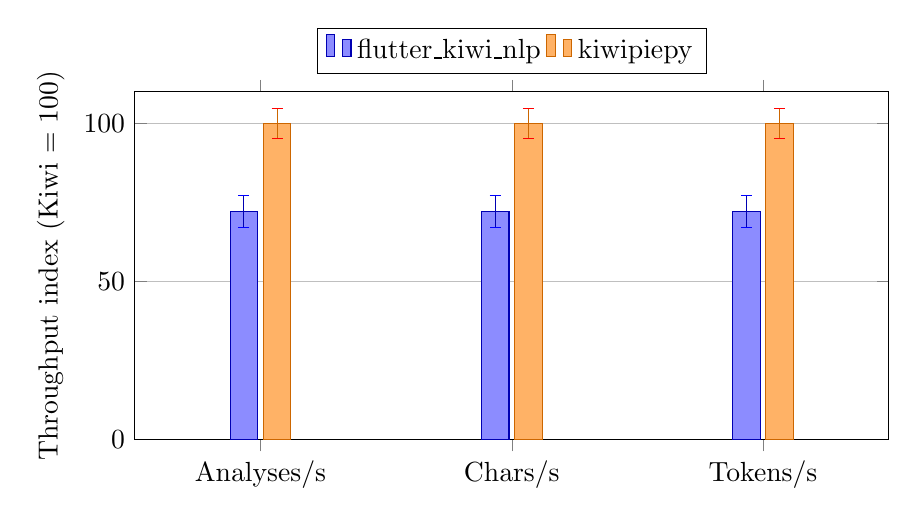
\begin{tikzpicture}
\begin{axis}[
  ybar,
  bar width=10pt,
  width=0.92\linewidth,
  height=6.0cm,
  ymin=0,
  ymax=110,
  ymajorgrids=true,
  ylabel={Throughput index (Kiwi = 100)},
  symbolic x coords={Analyses/s,Chars/s,Tokens/s},
  xtick=data,
  legend style={at={(0.5,1.05)}, anchor=south, legend columns=-1},
  enlarge x limits=0.25
]
\addplot+[
  fill=blue!45,
  draw=blue!70!black,
  error bars/.cd,
  y dir=both,
  y explicit
] coordinates {
  (Analyses/s,72.09) +- (0,5.07)
  (Chars/s,72.09) +- (0,5.07)
  (Tokens/s,72.20) +- (0,5.08)
};
\addplot+[
  fill=orange!60,
  draw=orange!80!black,
  error bars/.cd,
  y dir=both,
  y explicit
] coordinates {
  (Analyses/s,100.00) +- (0,4.75)
  (Chars/s,100.00) +- (0,4.75)
  (Tokens/s,100.00) +- (0,4.75)
};
\legend{flutter\_kiwi\_nlp,kiwipiepy}
\end{axis}
\end{tikzpicture}
\caption{Throughput comparison for macOS baseline (normalized index, mean ± stddev).}
\label{fig:throughput-index}
\end{figure}

\begin{figure}[htbp]
\centering
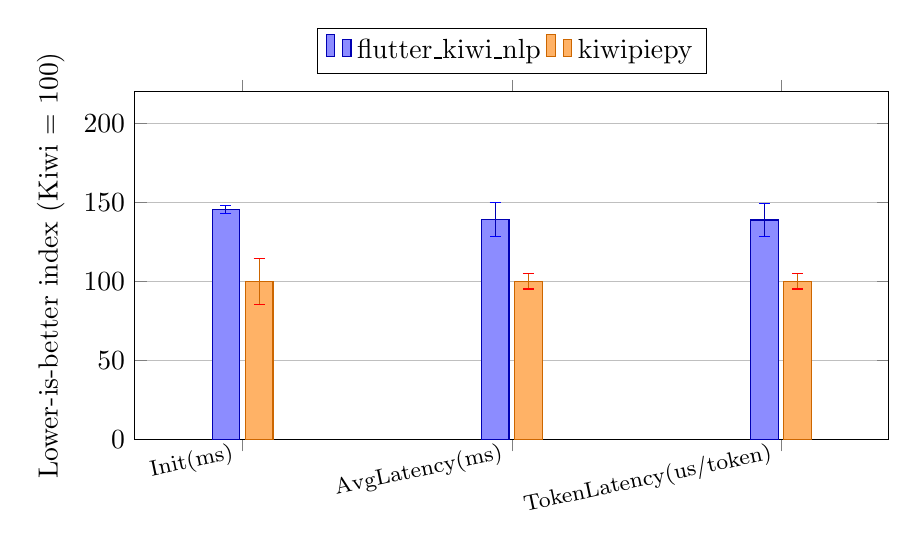
\begin{tikzpicture}
\begin{axis}[
  ybar,
  bar width=10pt,
  width=0.92\linewidth,
  height=6.0cm,
  ymin=0,
  ymax=220,
  ymajorgrids=true,
  ylabel={Lower-is-better index (Kiwi = 100)},
  symbolic x coords={Init(ms),AvgLatency(ms),TokenLatency(us/token)},
  xtick=data,
  x tick label style={font=\footnotesize, rotate=12, anchor=east},
  legend style={at={(0.5,1.05)}, anchor=south, legend columns=-1},
  enlarge x limits=0.20
]
\addplot+[
  fill=blue!45,
  draw=blue!70!black,
  error bars/.cd,
  y dir=both,
  y explicit
] coordinates {
  (Init(ms),145.53) +- (0,2.39)
  (AvgLatency(ms),139.08) +- (0,10.72)
  (TokenLatency(us/token),138.86) +- (0,10.70)
};
\addplot+[
  fill=orange!60,
  draw=orange!80!black,
  error bars/.cd,
  y dir=both,
  y explicit
] coordinates {
  (Init(ms),100.00) +- (0,14.65)
  (AvgLatency(ms),100.00) +- (0,4.76)
  (TokenLatency(us/token),100.00) +- (0,4.76)
};
\legend{flutter\_kiwi\_nlp,kiwipiepy}
\end{axis}
\end{tikzpicture}
\caption{Lower-is-better metrics for macOS baseline (normalized index, mean ± stddev).}
\label{fig:lower-better-index}
\end{figure}

\subsection{Per-Trial Raw Trace (Desktop Baseline)}
\begin{table}[htbp]
\centering
\caption{Per-trial raw snapshot for macOS baseline traceability}\label{tab:benchmark-trials}
\small
\begin{tabular}{@{}lrrrr@{}}
\toprule
Trial & Flutter init (ms) & Kiwi init (ms) & Flutter analyses/s & Kiwi analyses/s \\
\midrule
1 & 1423.93 & 810.77 & 2231.43 & 3316.65 \\
2 & 1387.41 & 1067.51 & 2615.10 & 3487.51 \\
3 & 1362.52 & 1114.31 & 2680.97 & 3669.04 \\
4 & 1404.55 & 815.85 & 2608.83 & 3456.25 \\
5 & 1385.88 & 976.95 & 2594.89 & 3731.77 \\
\bottomrule
\end{tabular}
\end{table}

\begin{figure}[htbp]
\centering
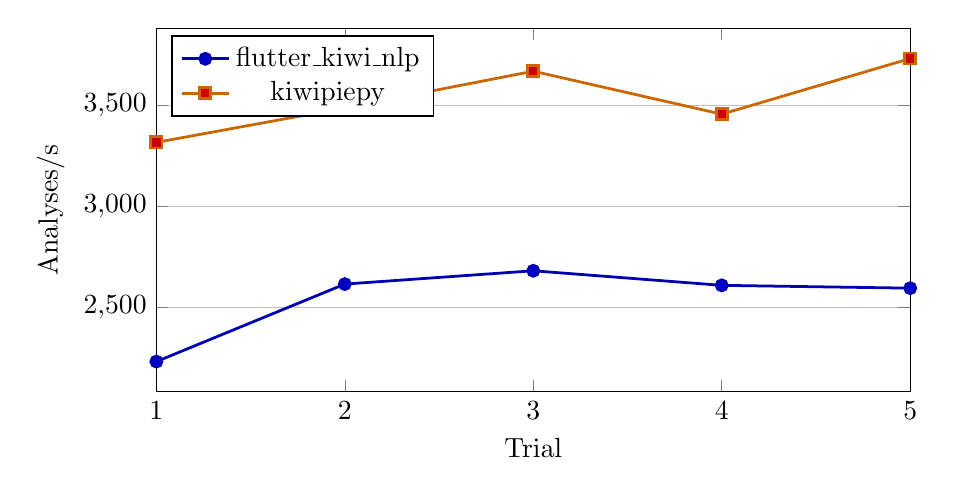
\begin{tikzpicture}
\begin{axis}[
  width=0.92\linewidth,
  height=6.2cm,
  xlabel={Trial},
  ylabel={Analyses/s},
  xmin=1,
  xmax=5,
  xtick={1,2,3,4,5},
  ymajorgrids=true,
  legend style={at={(0.02,0.98)}, anchor=north west}
]
\addplot+[
  color=blue!70!black,
  mark=*,
  line width=1pt
] coordinates {
  (1,2231.43)
  (2,2615.10)
  (3,2680.97)
  (4,2608.83)
  (5,2594.89)
};
\addplot+[
  color=orange!80!black,
  mark=square*,
  line width=1pt
] coordinates {
  (1,3316.65)
  (2,3487.51)
  (3,3669.04)
  (4,3456.25)
  (5,3731.77)
};
\legend{flutter\_kiwi\_nlp,kiwipiepy}
\end{axis}
\end{tikzpicture}
\caption{Trial-by-trial throughput trace for macOS baseline (analyses per second).}
\label{fig:trial-throughput}
\end{figure}

\FloatBarrier

\subsection{Detailed Interpretation (Honest Reading)}
Across desktop and mobile trial sets, warm-path throughput and latency are
consistently stable, and warm per-call latency remains sub-millisecond in these
configurations (roughly 0.3--0.6 ms). This matches the practical impression
that repeated in-app analysis is responsive after initialization. At the same
time, repeated measurements still show slower init and lower throughput on the
Flutter path relative to the Python reference runtime, with magnitude varying
by environment (desktop native, iOS simulator debug, Android emulator release).
Compared with the previous mobile rows in this report, the updated run profile
shows improved Flutter warm throughput on both mobile targets
(iOS: \(2065.58 \rightarrow 2422.31\) analyses/s, +17.27\%;
Android: \(1981.83 \rightarrow 2214.79\) analyses/s, +11.75\%),
while desktop warm throughput moved slightly downward
(\(2659.19 \rightarrow 2546.24\) analyses/s, -4.25\%).
The revised methodology therefore surfaces a more nuanced trend:
mobile warm-path behavior improved under the updated setup, but cross-runtime
gaps still remain.

New boundary-decomposed instrumentation (Table~\ref{tab:benchmark-boundary})
adds direct evidence for where overhead accumulates. Flutter boundary loss
(full JSON path vs pure processing path) is 11.23\% on desktop, 13.07\% on iOS
simulator, and 15.22\% on Android emulator, with per-analysis overhead of
roughly 0.05--0.10 ms.
This also bounds expected gains from JSON-path removal alone: eliminating
serialization would likely recover a meaningful fraction of warm-path overhead,
but not necessarily close the entire cross-runtime gap by itself.

Based on code inspection and payload values, the most likely contributors are:
\begin{enumerate}[leftmargin=1.5em]
  \item \textbf{Boundary conversion overhead (evidence-based):}
  native Flutter path returns JSON from C bridge
  (\texttt{flutter\_kiwi\_ffi\_analyze\_json}) and then parses it in Dart
  (\texttt{jsonDecode}). Python path consumes native results via a different
  binding stack without this exact JSON roundtrip. In bridge code, JSON is
  assembled through repeated \texttt{sb\_append(...)} operations and escaped
  field appends (\texttt{sb\_append\_json\_escaped}), which implies dynamic
  allocation/reallocation and additional O(n)-scale string-copy work on top of
  base inference.

  \item \textbf{Per-call async boundary cost (evidence-based):}
  Flutter benchmark loop awaits \texttt{Future} analysis call for each sentence,
  adding runtime overhead at Dart async/FFI boundaries.

  \item \textbf{Residual cross-runtime semantic gap (evidence-based):}
  this benchmark now passes explicit build and match bitmasks to both runtimes,
  reducing prior configuration mismatch risk. However, output token totals still
  differ (Flutter 9660 vs Python 9645), indicating backend-wrapper semantic
  differences even under aligned knobs.

  \item \textbf{Worker/thread auto mode mismatch (evidence-based):}
  both runtimes use auto settings (\texttt{-1}) for thread/worker counts, but
  auto-mode policies are not guaranteed to map to equivalent parallel execution
  strategy.
  \item \textbf{Model loading path variability (inference):}
  unless \texttt{--model-path} is forced, each runtime may initialize using
  different default lookup paths/caches, potentially affecting cold-start cost.
\end{enumerate}

\subsection{Threats to Validity}
Current benchmark limitations that should be stated explicitly:
\begin{itemize}[leftmargin=1.5em]
  \item Trial counts are improved but still modest for strong inference
  (desktop/iOS/Android all \texttt{n=5}).
  \item No explicit CPU pinning or thermal-state control.
  \item Bitmask parity is enforced, but internal backend semantics can still differ.
  \item Init metric combines multiple concerns (library load, model resolution,
  analyzer construction) rather than isolated micro-phases.
  \item iOS measurements in this report were collected on simulator in
  \texttt{debug} mode, because \texttt{release/profile} was unavailable in the
  current simulator setup.
  \item iOS simulator reports host-shared CPU/memory context
  (10 cores, 16 GiB RAM).
  \item These values are not equivalent to physical-device thermal or power
  constraints.
  \item Android measurements were collected on emulator, not on real devices.
  \item Android emulator guest was configured with 4 vCPUs and 2 GiB RAM, which
  can amplify startup variance and may not represent flagship physical devices.
  \item For mobile rows, \texttt{kiwipiepy} values come from host macOS runtime;
  therefore cross-runtime ratios on mobile rows should be interpreted as
  engineering reference, not strict same-device head-to-head evidence.
  \item Web runtime functionality is validated in tests, but sustained web
  throughput benchmark numbers are not included in this report.
  \item Gold-corpus quality evaluation in this revision covers two Kiwi-provided
  evaluation sets (191 sentences total). Broader domain coverage still requires
  larger and more heterogeneous corpora.
\end{itemize}

\subsection{Gold-Corpus Linguistic Agreement Evaluation}
To close the prior quality-evidence gap, this revision adds a reproducible
gold-corpus evaluation using:
\begin{itemize}[leftmargin=1.5em]
  \item \path{example/assets/gold\_eval\_web\_ko.txt} (158 sentences),
  \item \path{example/assets/gold\_eval\_written\_ko.txt} (33 sentences),
  \item shared options for both runtimes:
  \texttt{top\_n=1} and \texttt{build\_options=1039}.
  \item match options:
  \texttt{create\_match\_options=8454175} and
  \texttt{analyze\_match\_options=8454175}.
\end{itemize}

Evaluation command:
\begin{lstlisting}[style=code]
uv run python tool/benchmark/gold_corpus_compare.py \
  --device macos --mode release
\end{lstlisting}

Metrics are sequence-level agreements based on normalized Levenshtein distance:
token agreement compares \texttt{form} sequences, POS agreement compares
\texttt{form/tag} sequences, and sentence exact match requires full sequence
identity.
Let \(M\) be the number of evaluated sentences. For sentence \(i\),
\(g_i^{\mathrm{form}}\) and \(p_i^{\mathrm{form}}\) are gold/predicted token-form
sequences, and \(g_i^{\mathrm{pair}}\), \(p_i^{\mathrm{pair}}\) are gold/predicted
\texttt{form/tag} pair sequences.
\[
A_{\mathrm{token}}
=1-\frac{
\sum_{i=1}^{M} d_{\mathrm{Lev}}(g_i^{\mathrm{form}},p_i^{\mathrm{form}})
}{
\sum_{i=1}^{M} \max\!\left(
\left|g_i^{\mathrm{form}}\right|,\left|p_i^{\mathrm{form}}\right|
\right)
}.
\]
\[
A_{\mathrm{pos}}
=1-\frac{
\sum_{i=1}^{M} d_{\mathrm{Lev}}(g_i^{\mathrm{pair}},p_i^{\mathrm{pair}})
}{
\sum_{i=1}^{M} \max\!\left(
\left|g_i^{\mathrm{pair}}\right|,\left|p_i^{\mathrm{pair}}\right|
\right)
}.
\]
\[
E_{\mathrm{token-seq}}
=\frac{1}{M}\sum_{i=1}^{M}\mathbf{1}\!\left[
g_i^{\mathrm{form}}=p_i^{\mathrm{form}}
\right],\quad
E_{\mathrm{sentence}}
=\frac{1}{M}\sum_{i=1}^{M}\mathbf{1}\!\left[
g_i^{\mathrm{pair}}=p_i^{\mathrm{pair}}
\right].
\]

\begin{table}[htbp]
\centering
\caption{Gold-corpus overall agreement (191 sentences, 7,990 gold tokens)}
\label{tab:gold-overall}
\begin{tabular}{@{}lrrr@{}}
\toprule
Metric & flutter\_kiwi\_nlp & kiwipiepy & Delta (pp) \\
\midrule
Token agreement & 88.39\% & 88.58\% & -0.19 \\
POS agreement & 84.90\% & 85.55\% & -0.65 \\
Token-sequence exact match & 3.66\% & 3.66\% & +0.00 \\
Sentence exact match & 1.57\% & 2.62\% & -1.05 \\
\bottomrule
\end{tabular}
\end{table}

\begin{table}[htbp]
\centering
\small
\caption{Per-dataset agreement breakdown}
\label{tab:gold-datasets}
\begin{tabular}{@{}llrrrr@{}}
\toprule
Dataset & Runtime & Token (\%) & POS (\%) & Token exact (\%) & Sentence exact (\%) \\
\midrule
web\_ko & flutter\_kiwi\_nlp & 87.79 & 84.04 & 3.80 & 1.90 \\
web\_ko & kiwipiepy & 88.03 & 84.80 & 3.80 & 2.53 \\
written\_ko & flutter\_kiwi\_nlp & 90.86 & 88.42 & 3.03 & 0.00 \\
written\_ko & kiwipiepy & 90.86 & 88.61 & 3.03 & 3.03 \\
\bottomrule
\end{tabular}
\end{table}

\begin{figure}[htbp]
\centering
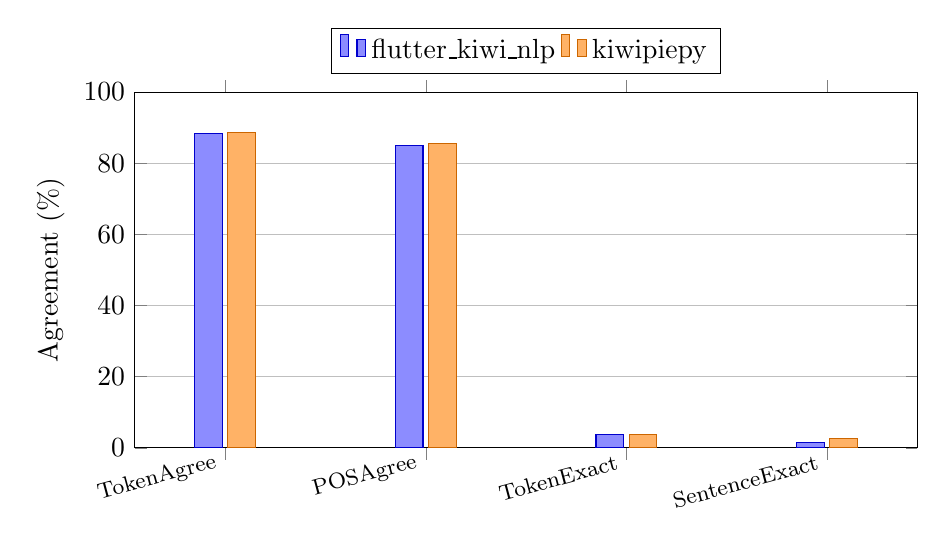
\begin{tikzpicture}
\begin{axis}[
  ybar,
  bar width=10pt,
  width=0.95\linewidth,
  height=6.1cm,
  ymin=0,
  ymax=100,
  ymajorgrids=true,
  ylabel={Agreement (\%)},
  symbolic x coords={TokenAgree,POSAgree,TokenExact,SentenceExact},
  xtick=data,
  x tick label style={font=\footnotesize, rotate=15, anchor=east},
  legend style={at={(0.5,1.05)}, anchor=south, legend columns=-1},
  enlarge x limits=0.15
]
\addplot+[fill=blue!45,draw=blue!80!black] coordinates {
  (TokenAgree,88.39)
  (POSAgree,84.90)
  (TokenExact,3.66)
  (SentenceExact,1.57)
};
\addplot+[fill=orange!60,draw=orange!80!black] coordinates {
  (TokenAgree,88.58)
  (POSAgree,85.55)
  (TokenExact,3.66)
  (SentenceExact,2.62)
};
\legend{flutter\_kiwi\_nlp,kiwipiepy}
\end{axis}
\end{tikzpicture}
\caption{Overall gold-corpus agreement metrics across runtimes.}
\label{fig:gold-overall}
\end{figure}

\begin{figure}[htbp]
\centering
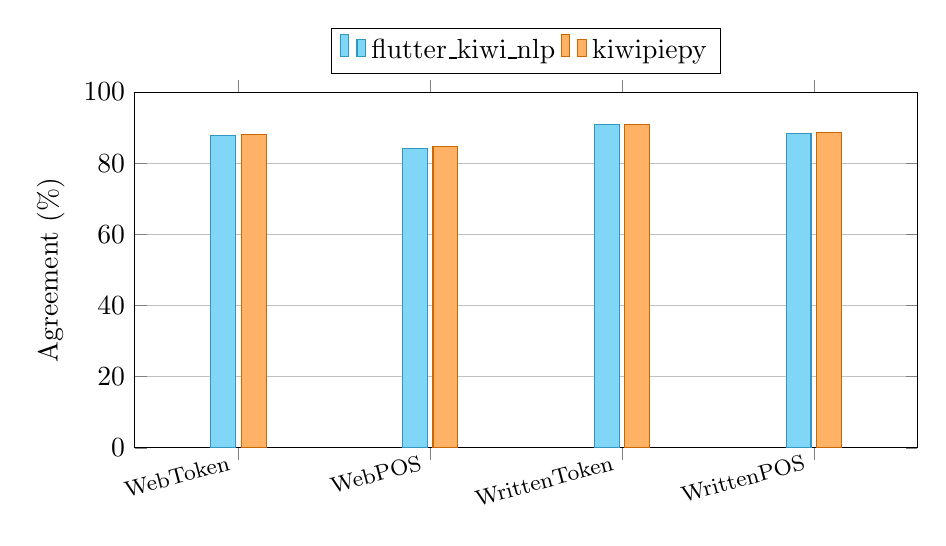
\begin{tikzpicture}
\begin{axis}[
  ybar,
  bar width=9pt,
  width=0.95\linewidth,
  height=6.1cm,
  ymin=0,
  ymax=100,
  ymajorgrids=true,
  ylabel={Agreement (\%)},
  symbolic x coords={WebToken,WebPOS,WrittenToken,WrittenPOS},
  xtick=data,
  x tick label style={font=\footnotesize, rotate=15, anchor=east},
  legend style={at={(0.5,1.05)}, anchor=south, legend columns=-1},
  enlarge x limits=0.18
]
\addplot+[fill=cyan!50,draw=cyan!75!black] coordinates {
  (WebToken,87.79)
  (WebPOS,84.04)
  (WrittenToken,90.86)
  (WrittenPOS,88.42)
};
\addplot+[fill=orange!60,draw=orange!80!black] coordinates {
  (WebToken,88.03)
  (WebPOS,84.80)
  (WrittenToken,90.86)
  (WrittenPOS,88.61)
};
\legend{flutter\_kiwi\_nlp,kiwipiepy}
\end{axis}
\end{tikzpicture}
\caption{Per-dataset token/POS agreement profile.}
\label{fig:gold-dataset-token-pos}
\end{figure}

\begin{figure}[htbp]
\centering
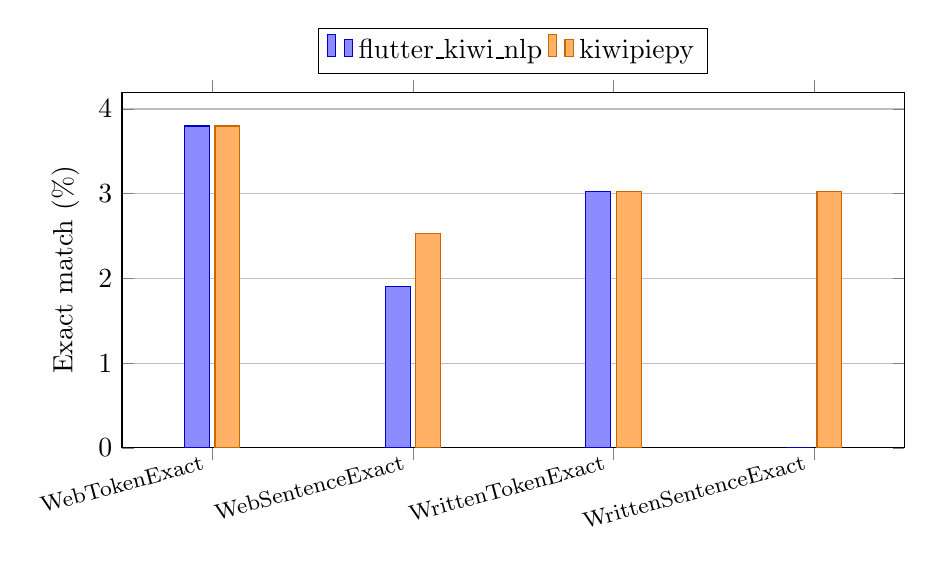
\begin{tikzpicture}
\begin{axis}[
  ybar,
  bar width=9pt,
  width=0.95\linewidth,
  height=6.1cm,
  ymin=0,
  ymax=4.2,
  ymajorgrids=true,
  ylabel={Exact match (\%)},
  symbolic x coords={WebTokenExact,WebSentenceExact,WrittenTokenExact,WrittenSentenceExact},
  xtick=data,
  x tick label style={font=\footnotesize, rotate=15, anchor=east},
  legend style={at={(0.5,1.05)}, anchor=south, legend columns=-1},
  enlarge x limits=0.15
]
\addplot+[fill=blue!45,draw=blue!80!black] coordinates {
  (WebTokenExact,3.80)
  (WebSentenceExact,1.90)
  (WrittenTokenExact,3.03)
  (WrittenSentenceExact,0.00)
};
\addplot+[fill=orange!60,draw=orange!80!black] coordinates {
  (WebTokenExact,3.80)
  (WebSentenceExact,2.53)
  (WrittenTokenExact,3.03)
  (WrittenSentenceExact,3.03)
};
\legend{flutter\_kiwi\_nlp,kiwipiepy}
\end{axis}
\end{tikzpicture}
\caption{Exact-match comparison on gold corpora (strict full-sequence criteria).}
\label{fig:gold-exact}
\end{figure}

\subsection{Interpretation of Gold-Corpus Results}
Aggregate token and POS agreement are close between runtimes (sub-1pp gap), but
strict sentence exact match remains low on both sides. This is expected for
Korean morphological pipelines where small boundary/tag normalization differences
across wrappers can fail whole-sentence exactness despite high token-level
agreement. The combined predicted token totals (Flutter 8,076; Kiwi 8,103)
confirm minor segmentation divergence under aligned option bitmasks.

\subsection{Recommended Protocol for Fairer Future Comparisons}
\begin{enumerate}[leftmargin=1.5em]
  \item Force same model assets by passing identical absolute
  \texttt{--model-path}.
  \item Keep explicit bitmask parity and additionally validate per-sentence
  output equivalence for sampled cases.
  \item Run repeated trials (for example 10+), report mean/median/stddev.
  \item Separate measurements into cold init, warm init, and steady-state
  analysis throughput.
  \item Record exact binary/model versions in output payload metadata.
\end{enumerate}

\section{Security and Supply-Chain Considerations}
\subsection{Archive Integrity}
Both native and web fallback flows support optional SHA-256 verification, which
is critical when model archives are downloaded at runtime.

\subsection{Web CSP and CDN Trust Boundary}
By default, web runtime bootstrap uses CDN-hosted \texttt{kiwi-nlp} module and
WASM URLs (jsDelivr) unless overridden through
\path{FLUTTER_KIWI_NLP_WEB_MODULE_URL} and
\path{FLUTTER_KIWI_NLP_WEB_WASM_URL}. Production deployments therefore
need explicit Content Security Policy (CSP) allowances for the selected module
and WASM origins (or must self-host these artifacts under an already-allowed
origin). This CDN trust boundary is distinct from model-archive integrity checks.

\subsection{Dynamic Loading Risk}
Environment-based dynamic library overrides are useful for controlled deployment,
but should be restricted in hardened environments to avoid untrusted path
injection.

\subsection{Failure Transparency}
The plugin intentionally prefers explicit hard failure with context-rich errors
instead of silent fallback. This behavior improves diagnosability and reduces
risk of undetected incorrect execution.

\section{Maintainability Notes}
\subsection{Separation of Concerns}
\begin{itemize}[leftmargin=1.5em]
  \item Public API and models are compact and typed.
  \item Runtime-specific logic is isolated in dedicated files
  (native, web, stub).
  \item Shared model-file metadata and validation helpers are centralized in
  \texttt{kiwi\_model\_assets.dart}.
\end{itemize}

\subsection{Testability Hooks}
Native analyzer exposes explicit debug hooks for tests:

\begin{itemize}[leftmargin=1.5em]
  \item binding factory override,
  \item archive URL/checksum override,
  \item HTTP client factory override.
\end{itemize}

These hooks allow deterministic tests for initialization and fallback branches.

\section{Testing and Coverage Quality}
\subsection{Test Suite Scope}
As of February 18, 2026, the test suite is organized in layered form:
\begin{itemize}[leftmargin=1.5em]
  \item Core package layer (\path{test/}): 63 unit tests in 14 groups across
  9 files.
  \item Example widget/golden layer (\path{example/test/}): 5 tests, including
  3 screenshot(golden) assertions.
  \item Example integration/acceptance layer
  (\path{example/integration\_test/}): 3 end-to-end tests.
\end{itemize}

This yields 71 test declarations across repository test directories. Coverage
focus in the core package layer remains strongest on API contract behavior,
typed model parsing, option flags, error semantics, and native fallback logic.
For macOS desktop execution, the three integration tests pass under serial
invocation with explicit device pinning (\texttt{-d macos}).

Key tested areas include:
\begin{itemize}[leftmargin=1.5em]
  \item public API export and unsupported-platform behavior,
  \item native analyzer lifecycle (\texttt{create}/\texttt{analyze}/
  \texttt{addUserWord}/\texttt{close}),
  \item model path resolution and asset/archive fallback branches,
  \item JSON model decoding for \texttt{KiwiToken}, \texttt{KiwiCandidate},
  and \texttt{KiwiAnalyzeResult},
  \item option constant composition and exception formatting,
  \item acceptance flow over analyzer demo UI actions
  (analyze/clear/settings/POS-sheet),
  \item runtime smoke checks for \texttt{create} $\rightarrow$
  \texttt{analyze} $\rightarrow$ \texttt{close},
  \item native runtime-path probing on macOS FFI candidate resolution,
  \item screenshot(golden) stability checks for settings and POS dictionary
  sheets under a fixed mobile viewport.
\end{itemize}

\subsection{Coverage Snapshot}
Using \texttt{flutter test --coverage test} on February 18, 2026
(core package layer only):
\begin{itemize}[leftmargin=1.5em]
  \item Raw line coverage: 384/384 = 100.00\%.
  \item Filtered line coverage: 81/81 = 100.00\%.
\end{itemize}

Compared with the previous paper snapshot (raw 93.58\%), raw line coverage
improves by +6.42 percentage points in this revision.

\begin{figure}[htbp]
\centering
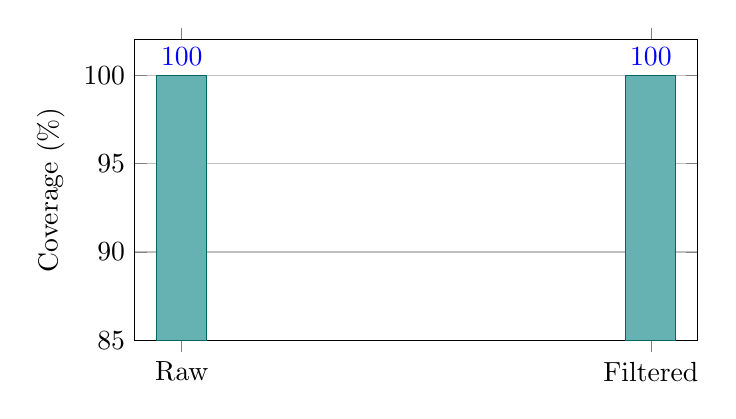
\begin{tikzpicture}
\begin{axis}[
  ybar,
  bar width=18pt,
  width=0.72\linewidth,
  height=5.4cm,
  ymin=85,
  ymax=102,
  ymajorgrids=true,
  ylabel={Coverage (\%)},
  symbolic x coords={Raw,Filtered},
  xtick=data,
  nodes near coords,
  nodes near coords align={vertical}
]
\addplot+[fill=teal!60, draw=teal!80!black] coordinates {
  (Raw,100.00)
  (Filtered,100.00)
};
\end{axis}
\end{tikzpicture}
\caption{Coverage snapshot used in this paper.}
\label{fig:coverage-bars}
\end{figure}

\FloatBarrier

\subsection{Why Raw and Filtered Coverage Can Differ}
The project includes a filtered coverage gate
(\texttt{tool/check\_coverage.sh}) that excludes:
\begin{itemize}[leftmargin=1.5em]
  \item generated binding file:\newline
  \path{lib/flutter_kiwi_ffi_bindings_generated.dart},
  \item native runtime implementation:\newline
  \path{lib/src/kiwi_analyzer_native.dart},
  \item web runtime implementation:\newline
  \path{lib/src/kiwi_analyzer_web.dart}.
\end{itemize}

The rationale is that parts of these files require runtime/platform integration
contexts that are harder to exercise in hermetic unit tests. This makes
filtered coverage useful as a strict gate for stable pure-Dart layers, but it
must not be interpreted as full end-to-end runtime coverage. In the current
snapshot, raw and filtered values are equal (both 100.00\%), but the filtered
gate remains relevant as a policy mechanism for future regressions.

\subsection{Honest Quality Assessment}
The present quality state is strong for deterministic unit-level contract tests
and includes expanded acceptance/golden coverage in the example app.
Remaining risk still concentrates in integration boundaries:
\begin{itemize}[leftmargin=1.5em]
  \item native dynamic loading and ABI interaction across target platforms,
  \item web module import/WASM loading under browser/network constraints,
  \item platform build-hook behavior in real CI/device matrices,
  \item physical mobile device variability beyond simulator/emulator
  environments.
\end{itemize}

Therefore, line coverage should be treated as one quality indicator, not a
complete reliability proof. Integration tests on actual target runtimes are the
next quality multiplier for this plugin class.

\section{Limitations and Future Work}
\subsection{Current Limitations}
\begin{itemize}[leftmargin=1.5em]
  \item Web runtime depends on module/WASM artifact availability unless
  module, WASM, and model assets are self-hosted under
  application-controlled origins.
  \item Web deployments must satisfy CSP rules for module/WASM fetch origins.
  Because the default bootstrap uses CDN URLs, this creates an explicit
  supply-chain boundary unless deployments self-host artifacts.
  \item Native archive fallback requires network access and writable cache
  location when model assets are not bundled locally.
  \item Throughput can trail Python-native execution in current measurements;
  a major contributor is bridge-level JSON serialization overhead in the native
  C layer (dynamic allocation and string copy cost on hot paths).
  \item Native execution is in-process via FFI; a crash in dependent native
  code is fatal to the host Flutter process (no process isolation boundary).
  \item Platforms outside declared plugin matrix are unsupported.
  \item Current mobile benchmark rows use simulator/emulator environments
  (iOS debug simulator, Android emulator), not physical iOS/Android devices.
  \item Web throughput benchmark rows are not yet included in this report.
\end{itemize}

\subsection{Clarifications on Common Reviewer Questions}
\begin{itemize}[leftmargin=1.5em]
  \item \textbf{Could zero-copy or binary bridge close the 0.72x gap?}
  It is a promising direction and is explicitly planned. Current boundary
  measurements indicate JSON-path overhead around 11--15\% on warm paths; this
  suggests meaningful gains, but also implies that non-JSON residual costs may
  still remain after migration.
  \item \textbf{Does Android init include asset extraction from APK?}
  Yes, the reported init metric wraps \texttt{KiwiAnalyzer.create(...)} and can
  include model-path resolution and asset-copy work on cache-miss paths, in
  addition to native bridge/Kiwi initialization.
  \item \textbf{How is Web TTI impacted by WASM/model download size?}
  First-use web latency is affected by module/WASM/model fetch and runtime
  instantiation; this report currently does not provide controlled TTI numbers,
  and therefore treats them as explicit future benchmarking scope.
\end{itemize}

\subsection{Recommended Future Work}\label{sec:future-work}
\begin{enumerate}[leftmargin=1.5em]
  \item \textbf{Bridge performance redesign:} prototype and A/B evaluate binary
  payload designs (for example FlatBuffers/Protobuf-style schemas) and typed
  native transfer paths against current JSON baseline. Report per-phase gains
  (serialize/parse/call boundary) and safety complexity (ownership/lifetime).
  \item \textbf{Benchmark external validity:} add release/profile measurements
  on physical iOS and Android devices, with repeated runs under thermal-state
  controls and explicit startup-path annotations (asset-cache hit/miss). Include
  sustained Web throughput plus first-use TTI rows under controlled
  network/cache conditions.
  \item \textbf{Operational hardening:} provide first-class self-hosting
  recipes for web module/WASM/model assets, with CSP and integrity examples.
  \item \textbf{Reliability engineering:} evaluate optional crash-containment
  architectures for native execution (for example, process separation modes for
  fault-intolerant deployments).
  \item \textbf{Compatibility governance:} expand CI validation across Kiwi
  versions/model families and platform-specific binary packaging combinations.
  \item \textbf{Quality expansion:} add deterministic regression fixtures for
  hard tokenization/POS edge cases and broaden integration tests on real target
  runtimes.
  \item \textbf{API evolution:} assess optional batch-analysis APIs for
  high-throughput service scenarios without breaking existing contracts.
\end{enumerate}

\section{Conclusion}
\texttt{flutter\_kiwi\_nlp} contributes a native-first, cross-platform
integration architecture that exposes one stable Dart API while spanning two
runtime stacks (native FFI and web WASM). The implementation focus is practical
deployment quality: explicit fallback order, reproducible build hooks, typed
result contracts, and diagnosable failure behavior.

Empirical evidence in this paper indicates three core outcomes. First, runtime
semantics are operationally aligned across targets under a shared API model.
Second, the package is suitable for on-device and offline-native inference
workflows once required model assets are provisioned locally. Third, current
performance trade-offs are transparent: Flutter-path throughput can trail the
Python baseline in measured settings, with bridge serialization overhead and
runtime-context differences as key contributors.
The updated benchmark revision further shows that mobile warm-path throughput
can improve under tuned run settings while boundary-decomposed profiling still
identifies a persistent JSON-path penalty (roughly 11--15\% in this report).

This paper intentionally does not claim a new morphology model or SOTA language
accuracy contribution. Its contribution is systems engineering: making Kiwi
usable in production Flutter applications across Android, iOS, macOS, Linux,
Windows, and Web with explicit operational contracts.

For practitioners, the key value is reduced integration risk when one codebase
must ship across platforms while preserving deterministic Korean NLP behavior.
For researchers and reviewers, the value is a reproducible, implementation-level
specification that surfaces both strengths and unresolved constraints.

\sloppy
\begin{thebibliography}{99}
\bibitem{ref_bert}
J. Devlin, M.-W. Chang, K. Lee, and K. Toutanova, ``BERT: Pre-training of Deep
Bidirectional Transformers for Language Understanding,'' arXiv preprint
arXiv:1810.04805, 2018. [Online]. Available:
\url{https://arxiv.org/abs/1810.04805}. [Accessed: 2026-02-17].

\bibitem{ref_albert}
Z. Lan, M. Chen, S. Goodman, K. Gimpel, P. Sharma, and R. Soricut, ``ALBERT:
A Lite BERT for Self-supervised Learning of Language Representations,'' arXiv
preprint arXiv:1909.11942, 2019. [Online]. Available:
\url{https://arxiv.org/abs/1909.11942}. [Accessed: 2026-02-17].

\bibitem{ref_electra}
K. Clark, M.-T. Luong, Q. V. Le, and C. D. Manning, ``ELECTRA: Pre-training
Text Encoders as Discriminators Rather Than Generators,'' arXiv preprint
arXiv:2003.10555, 2020. [Online]. Available:
\url{https://arxiv.org/abs/2003.10555}. [Accessed: 2026-02-17].

\bibitem{ref_distilbert}
V. Sanh, L. Debut, J. Chaumond, and T. Wolf, ``DistilBERT, a distilled
version of BERT: smaller, faster, cheaper and lighter,'' arXiv preprint
arXiv:1910.01108, 2019. [Online]. Available:
\url{https://arxiv.org/abs/1910.01108}. [Accessed: 2026-02-17].

\bibitem{ref_tinybert}
X. Jiao, Y. Yin, L. Shang, X. Jiang, X. Chen, L. Li, F. Wang, and Q. Liu,
``TinyBERT: Distilling BERT for Natural Language Understanding,'' arXiv
preprint arXiv:1909.10351, 2019. [Online]. Available:
\url{https://arxiv.org/abs/1909.10351}. [Accessed: 2026-02-17].

\bibitem{ref_minilm}
W. Wang, F. Wei, L. Dong, H. Bao, N. Yang, and M. Zhou, ``MiniLM: Deep
Self-Attention Distillation for Task-Agnostic Compression of Pre-Trained
Transformers,'' arXiv preprint arXiv:2002.10957, 2020. [Online]. Available:
\url{https://arxiv.org/abs/2002.10957}. [Accessed: 2026-02-17].

\bibitem{ref_mobilebert}
Z. Sun, H. Yu, X. Song, R. Liu, Y. Yang, and D. Zhou, ``MobileBERT: a Compact
Task-Agnostic BERT for Resource-Limited Devices,'' arXiv preprint
arXiv:2004.02984, 2020. [Online]. Available:
\url{https://arxiv.org/abs/2004.02984}. [Accessed: 2026-02-17].

\bibitem{ref_squeezebert}
F. N. Iandola, A. E. Shaw, R. Krishna, and K. W. Keutzer, ``SqueezeBERT: What
can computer vision teach NLP about efficient neural networks?'' arXiv
preprint arXiv:2006.11316, 2020. [Online]. Available:
\url{https://arxiv.org/abs/2006.11316}. [Accessed: 2026-02-17].

\bibitem{ref_edgebert}
T. Tambe et al., ``EdgeBERT: Sentence-Level Energy Optimizations for
Latency-Aware Multi-Task NLP Inference,'' arXiv preprint arXiv:2011.14203,
2020. [Online]. Available: \url{https://arxiv.org/abs/2011.14203}. [Accessed:
2026-02-17].

\bibitem{ref_deebert}
J. Xin, R. Tang, J. Lee, Y. Yu, and J. Lin, ``DeeBERT: Dynamic Early Exiting
for Accelerating BERT Inference,'' arXiv preprint arXiv:2004.12993, 2020.
[Online]. Available: \url{https://arxiv.org/abs/2004.12993}. [Accessed:
2026-02-17].

\bibitem{ref_pnlp_mixer}
F. Fusco, D. Pascual, P. Staar, and D. Antognini, ``pNLP-Mixer: an Efficient
all-MLP Architecture for Language,'' arXiv preprint arXiv:2202.04350, 2022.
[Online]. Available: \url{https://arxiv.org/abs/2202.04350}. [Accessed:
2026-02-17].

\bibitem{ref_on_device_apps}
N. Goyal, ``A comprehensive study of on-device NLP applications -- VQA,
automated Form filling, Smart Replies for Linguistic Codeswitching,'' arXiv
preprint arXiv:2409.19010, 2024. [Online]. Available:
\url{https://arxiv.org/abs/2409.19010}. [Accessed: 2026-02-17].

\bibitem{ref_personalized_vocab}
S. Wang, A. Shenoy, P. Chuang, and J. Nguyen, ``Now It Sounds Like You:
Learning Personalized Vocabulary On Device,'' arXiv preprint
arXiv:2305.03584, 2023. [Online]. Available:
\url{https://arxiv.org/abs/2305.03584}. [Accessed: 2026-02-17].

\bibitem{ref_kr_bert}
S. Lee, H. Jang, Y. Baik, S. Park, and H. Shin, ``KR-BERT: A Small-Scale
Korean-Specific Language Model,'' arXiv preprint arXiv:2008.03979, 2020.
[Online]. Available: \url{https://arxiv.org/abs/2008.03979}. [Accessed:
2026-02-17].

\bibitem{ref_klue}
S. Park et al., ``KLUE: Korean Language Understanding Evaluation,'' arXiv
preprint arXiv:2105.09680, 2021. [Online]. Available:
\url{https://arxiv.org/abs/2105.09680}. [Accessed: 2026-02-17].

\bibitem{ref_kobigbird}
K. Yang, Y. Jang, T. Lee, J. Seong, H. Lee, H. Jang, and H. Lim,
``KoBigBird-large: Transformation of Transformer for Korean Language
Understanding,'' arXiv preprint arXiv:2309.10339, 2023. [Online]. Available:
\url{https://arxiv.org/abs/2309.10339}. [Accessed: 2026-02-17].

\bibitem{ref_korean_morph_pos}
A. Matteson, C. Lee, Y.-B. Kim, and H. Lim, ``Rich Character-Level Information
for Korean Morphological Analysis and Part-of-Speech Tagging,'' arXiv preprint
arXiv:1806.10771, 2018. [Online]. Available:
\url{https://arxiv.org/abs/1806.10771}. [Accessed: 2026-02-17].

\bibitem{ref_mecab_ko}
T. Kudo, ``MeCab: Yet Another Part-of-Speech and Morphological Analyzer,''
[Online]. Available: \url{https://taku910.github.io/mecab/}. [Accessed:
2026-02-17].

\bibitem{ref_mecab_ko_dic}
Eunjeon Project, ``Eunjeon Korean NLP project page (MeCab-ko lineage),'' Blog.
[Online]. Available: \url{http://eunjeon.blogspot.com/}. [Accessed:
2026-02-17].

\bibitem{ref_khaiii}
Kakao Corp., ``Khaiii repository,'' GitHub. [Online]. Available:
\url{https://github.com/kakao/khaiii}. [Accessed: 2026-02-17].

\bibitem{ref_konlpy}
KoNLPy Contributors, ``KoNLPy documentation,'' [Online]. Available:
\url{https://konlpy.org/en/latest/}. [Accessed: 2026-02-17].

\bibitem{ref_github_rest}
GitHub Docs, ``GitHub REST API documentation.'' [Online]. Available:
\url{https://docs.github.com/en/rest}. [Accessed: 2026-02-17].




\bibitem{ref_kiwi_repo}
bab2min, ``Kiwi repository,'' GitHub. [Online]. Available:
\url{https://github.com/bab2min/Kiwi}. [Accessed: 2026-02-17].

\bibitem{ref_open_korean_text}
Open Korean Text Contributors, ``Open Korean Text repository,'' GitHub.
[Online]. Available: \url{https://github.com/open-korean-text/open-korean-text}.
[Accessed: 2026-02-17].

\bibitem{ref_komoran_repo}
SHINEWARE, ``KOMORAN repository,'' GitHub. [Online]. Available:
\url{https://github.com/shineware/KOMORAN}. [Accessed: 2026-02-17].

\bibitem{ref_konlpy_repo}
KoNLPy Contributors, ``KoNLPy repository,'' GitHub. [Online]. Available:
\url{https://github.com/konlpy/konlpy}. [Accessed: 2026-02-17].

\bibitem{ref_glue}
A. Wang, A. Singh, J. Michael, F. Hill, O. Levy, and S. R. Bowman, ``GLUE:
A Multi-Task Benchmark and Analysis Platform for Natural Language
Understanding,'' arXiv preprint arXiv:1804.07461, 2018. [Online]. Available:
\url{https://arxiv.org/abs/1804.07461}. [Accessed: 2026-02-17].

\bibitem{ref_superglue}
A. Wang et al., ``SuperGLUE: A Stickier Benchmark for General-Purpose Language
Understanding Systems,'' arXiv preprint arXiv:1905.00537, 2019. [Online].
Available: \url{https://arxiv.org/abs/1905.00537}. [Accessed: 2026-02-17].

\bibitem{ref_lra}
Y. Tay et al., ``Long Range Arena: A Benchmark for Efficient Transformers,''
arXiv preprint arXiv:2011.04006, 2020. [Online]. Available:
\url{https://arxiv.org/abs/2011.04006}. [Accessed: 2026-02-17].

\bibitem{ref_dawnbench}
C. Coleman et al., ``Analysis of DAWNBench, a Time-to-Accuracy Machine Learning
Performance Benchmark,'' arXiv preprint arXiv:1806.01427, 2018. [Online].
Available: \url{https://arxiv.org/abs/1806.01427}. [Accessed: 2026-02-17].

\bibitem{ref_mlperf_inference}
V. J. Reddi et al., ``MLPerf Inference Benchmark,'' arXiv preprint
arXiv:1911.02549, 2019. [Online]. Available:
\url{https://arxiv.org/abs/1911.02549}. [Accessed: 2026-02-17].

\bibitem{ref_tinyml}
S. S. Chawathe et al., ``Tiny Machine Learning: Progress and Futures,'' arXiv
preprint arXiv:2403.19076, 2024. [Online]. Available:
\url{https://arxiv.org/abs/2403.19076}. [Accessed: 2026-02-17].

\bibitem{ref_fedavg}
H. B. McMahan et al., ``Communication-Efficient Learning of Deep Networks from
Decentralized Data,'' arXiv preprint arXiv:1602.05629, 2016. [Online]. Available:
\url{https://arxiv.org/abs/1602.05629}. [Accessed: 2026-02-17].
\bibitem{ref_kiwi_paper}
E. Park and S. Park, ``Kiwi: A Study on Developing a Korean Morphological
Analyzer,'' \textit{Korean Journal
of Digital Humanities}, vol. 1, no. 1, pp. 109--135, 2018. [Online].
Available: \url{https://accesson.kr/kjdh/v.1/1/109/43508}. [Accessed:
2026-02-17].

\bibitem{ref_kiwi_types_h}
bab2min, ``Kiwi model/type definitions (\texttt{include/kiwi/Types.h}),''
GitHub. [Online]. Available:
\url{https://github.com/bab2min/Kiwi/blob/main/include/kiwi/Types.h}.
[Accessed: 2026-02-17].

\bibitem{ref_kiwi_kiwi_h}
bab2min, ``Kiwi C++ API and model includes (\texttt{include/kiwi/Kiwi.h}),''
GitHub. [Online]. Available:
\url{https://github.com/bab2min/Kiwi/blob/main/include/kiwi/Kiwi.h}.
[Accessed: 2026-02-17].

\bibitem{ref_kiwi_path_evaluator}
bab2min, ``Kiwi path-scoring implementation (\texttt{src/PathEvaluator.hpp}),''
GitHub. [Online]. Available:
\url{https://github.com/bab2min/Kiwi/blob/main/src/PathEvaluator.hpp}.
[Accessed: 2026-02-17].

\end{thebibliography}

\appendix
\section{Appendix A: End-to-End Usage Example}
\begin{lstlisting}[style=code]
import 'package:flutter_kiwi_nlp/flutter_kiwi_nlp.dart';

Future<void> runSample() async {
  final KiwiAnalyzer analyzer = await KiwiAnalyzer.create(
    numThreads: -1,
    buildOptions: KiwiBuildOption.defaultOption,
    matchOptions: KiwiMatchOption.allWithNormalizing,
  );

  final KiwiAnalyzeResult result = await analyzer.analyze(
    'sample sentence for analysis',
    options: const KiwiAnalyzeOptions(topN: 1),
  );

  for (final KiwiCandidate candidate in result.candidates) {
    for (final KiwiToken token in candidate.tokens) {
      // Use token.form, token.tag, token.start, token.length, ...
    }
  }

  await analyzer.addUserWord('newword', tag: 'NNP', score: 1.0);
  await analyzer.close();
}
\end{lstlisting}

\section{Appendix B: Native and Web Runtime Equivalence Notes}
\begin{itemize}[leftmargin=1.5em]
  \item Method signatures are intentionally identical across native and web
  implementations.
  \item Result model shape is normalized to
  \texttt{KiwiAnalyzeResult -> KiwiCandidate -> KiwiToken}.
  \item Lifecycle rules are consistent: use-after-close triggers
  \texttt{KiwiException}.
  \item Web create-time handling of \texttt{numThreads}/\texttt{matchOptions}
  differs (accepted for parity, not applied at creation).
\end{itemize}

\section{Appendix C: Reproducibility Statement}
This report describes repository state and behavior as observed on
February 18, 2026. Build scripts, dependency versions, defaults, and benchmark
numbers may change in future releases. Formalized benchmark/testing pseudocode
is provided in Appendix D.

Minimal command sequence used for benchmark reproduction:
The measured mobile rows in this revision are simulator/emulator runs; physical
device command templates are included below for direct extension.
\begin{lstlisting}[style=code]
# Desktop baseline (macOS)
uv run python tool/benchmark/run_compare.py \
  --device macos --mode release --trials 5 \
  --warmup-runs 3 --measure-runs 15

# iOS simulator row (debug in this setup)
uv run python tool/benchmark/run_compare.py \
  --device "iPhone 17" --mode debug --trials 5 \
  --warmup-runs 3 --measure-runs 15

# Android emulator row (release)
uv run python tool/benchmark/run_compare.py \
  --device <android_emulator_id> --mode release --trials 5 \
  --warmup-runs 3 --measure-runs 15

# iOS physical device row (release; requires attached iPhone)
uv run python tool/benchmark/run_compare.py \
  --device <ios_physical_device_id> --mode release --trials 5 \
  --warmup-runs 3 --measure-runs 15

# Android physical device row (release; requires attached phone)
uv run python tool/benchmark/run_compare.py \
  --device <android_physical_device_id> --mode release --trials 5 \
  --warmup-runs 3 --measure-runs 15

# Core package unit tests (plugin root)
flutter test test

# Example screenshot(golden) tests (example app)
cd example
flutter test test/kiwi_ui_golden_test.dart

# Example integration/acceptance tests (run serially to avoid build.db lock)
flutter test integration_test/kiwi_runtime_smoke_test.dart -d macos
flutter test integration_test/kiwi_acceptance_flow_test.dart -d macos
flutter test integration_test/kiwi_native_runtime_path_test.dart -d macos
cd ..

# Gold-corpus agreement
uv run python tool/benchmark/gold_corpus_compare.py \
  --device macos --mode release

# Wrapper activity quantification snapshot
uv run python tool/benchmark/collect_wrapper_activity.py \
  --as-of-date 2026-02-17

# Environment capture used for Table "iOS/Android benchmark environment details"
flutter devices
sw_vers
sysctl -n machdep.cpu.brand_string
sysctl -n hw.ncpu
sysctl -n hw.memsize
xcodebuild -version
xcrun simctl list devices --json
xcrun simctl list runtimes --json
xcrun simctl list devicetypes --json
xcrun simctl spawn <ios_simulator_udid> /usr/sbin/sysctl -n hw.ncpu
xcrun simctl spawn <ios_simulator_udid> /usr/sbin/sysctl -n hw.memsize
adb -s <android_emulator_id> emu avd name
adb -s <android_emulator_id> shell getprop ro.build.version.sdk
adb -s <android_emulator_id> shell cat /proc/meminfo
adb -s <android_emulator_id> shell cat /proc/cpuinfo
cat ~/.android/avd/Pixel_9.avd/config.ini
\end{lstlisting}

Primary generated artifacts:
\begin{itemize}[leftmargin=1.5em]
  \item \path{benchmark/results/macos_release_t5_token_count_s10_v2/comparison.md}
  \item \path{benchmark/results/ios_debug_t5_token_count_s10_v2/comparison.md}
  \item \path{benchmark/results/android_release_t5_token_count_s10_v2/comparison.md}
  \item \path{benchmark/results/macos_release_t5_token_count_s10_v2/flutter_kiwi_benchmark_trials.json}
  \item \path{benchmark/results/macos_release_t5_token_count_s10_v2/kiwipiepy_benchmark_trials.json}
  \item \path{benchmark/results/gold_eval/comparison.md}
  \item \path{benchmark/results/gold_eval/flutter_overall.json}
  \item \path{benchmark/results/gold_eval/kiwipiepy_overall.json}
  \item \path{benchmark/results/wrapper_activity/wrapper_activity.json}
  \item \path{benchmark/results/wrapper_activity/wrapper_activity.md}
  \item per-trial JSON files for each runtime in \path{benchmark/results/}.
  \item screenshot(golden) baselines in
  \path{example/test/goldens/}.
\end{itemize}

\section{Appendix D: Benchmark and Test Execution Pseudocode}
\begin{figure}[t]
\caption{Cross-runtime benchmark orchestration
(\texttt{tool/benchmark/run\_compare.py})}
\label{alg:benchmark-orchestration}
\begin{algorithmic}[1]
\Require device $d$, mode $m$, corpus $p$, trials $n$, warmup $w$, measure $r$
\Ensure comparison report and per-trial JSON artifacts for Flutter and Python
\State Resolve output directory key from $(d,m,n,w,r)$ and options.
\For{$i \gets 1$ \textbf{to} $n$}
  \State Launch Flutter benchmark target
  \path{example/lib/benchmark_main.dart} on $(d,m)$.
  \State Wait for marker \texttt{KIWI\_BENCHMARK\_JSON=} in stdout.
  \If{marker is missing on Android}
    \State Scan \texttt{adb logcat} and reconstruct payload from base64 chunks.
  \EndIf
  \State Persist Flutter trial payload JSON.
  \State Run Python benchmark (\path{tool/benchmark/kiwipiepy_benchmark.py})
  with the same corpus and option bitmasks.
  \State Persist Python trial payload JSON.
\EndFor
\State Aggregate trial statistics (mean/stddev, ratio, per-trial snapshots).
\State Generate \path{comparison.md} via
\path{tool/benchmark/compare_results.py}.
\end{algorithmic}
\end{figure}

\begin{figure}[t]
\caption{Gold-corpus agreement evaluation
(\texttt{tool/benchmark/gold\_corpus\_compare.py})}
\label{alg:gold-corpus-eval}
\begin{algorithmic}[1]
\Require asset list $G$, device $d$, mode $m$, top-$N$, build/match options
\Ensure token/POS agreement metrics and dataset/overall JSON outputs
\ForAll{$g \in G$}
  \State Load tab-separated $(sentence, gold\_tokens)$ entries from $g$.
  \State Run Flutter evaluator target \path{example/lib/gold_eval_main.dart}.
  \State Parse \texttt{KIWI\_GOLD\_EVAL\_JSON=} payload.
  \State Run Python evaluator (\texttt{kiwipiepy}) with aligned options.
  \State Align outputs per sentence (top-1 candidate) and compute:
  token agreement, POS agreement, token-pair exact, sentence exact.
  \State Persist per-dataset JSON summaries.
\EndFor
\State Aggregate micro/macro overall metrics across datasets.
\State Emit
\path{benchmark/results/gold_eval/comparison.md},
\path{flutter_overall.json}, and \path{kiwipiepy_overall.json}.
\end{algorithmic}
\end{figure}

\begin{figure}[t]
\caption{Unit-test and coverage gate pipeline
(\texttt{tool/check\_coverage.sh})}
\label{alg:test-coverage-gate}
\begin{algorithmic}[1]
\Require repository root $R$, coverage threshold $\tau$ (default $100\%$)
\Ensure pass/fail decision with filtered coverage report
\State Execute \texttt{flutter test --coverage test}.
\If{\path{coverage/lcov.info} does not exist}
  \State \textbf{fail} with missing-report error.
\EndIf
\State Filter LCOV records, excluding generated/native/web runtime files.
\State Compute filtered coverage:
$\texttt{coverage} = 100 \times \texttt{LH}/\texttt{LF}$.
\State Write filtered report to \path{coverage/lcov.filtered.info}.
\If{$\texttt{coverage} < \tau$}
  \State \textbf{fail} coverage gate.
\Else
  \State \textbf{pass} and report filtered percentage.
\EndIf
\end{algorithmic}
\end{figure}

\end{document}
